\documentclass[10pt,a4paper]{memoir}

%%%%%%
% Preamble
%%%%%%
\usepackage{amssymb,amsmath,amssymb,amsthm} %Math stuff
\usepackage{graphicx} %Including images
\usepackage{epstopdf} %Useful if using pdflatex


\DeclareGraphicsRule{.tif}{png}{.png}{`convert #1 `dirname #1`/`basename #1 .tif`.png} %Used with the above

\renewcommand{\abstractnamefont}{\normalfont\Large\bfseries}%Formats abstract 
\renewcommand{\abstracttextfont}{\normalfont\normalsize}%Formats abstract

\newsubfloat{figure}%To use subfigures
\let\subfigure\subbottom

\bibliographystyle{alpha}%Bibliography style
%\bibliographystyle{plain}
\renewcommand{\bibname}{References}

%new commands

\newcommand{\rotation}{\mathbf{J}(\mathbf{\eta})}
\newcommand{\mass}{\mathbf{M}\mathbf{\dot{\nu}}}
\newcommand{\coriolis}{\mathbf{C}(\mathbf{\nu})\mathbf{\nu}}
\newcommand{\damping}{\mathbf{D}(\mathbf{\nu})\mathbf{\nu}}
\newcommand{\restoring}{\mathbf{G}(\mathbf{\eta})}
\newcommand{\force}{\mathbf{\tau}}

\newcommand{\interaction}{\mathbf{L}(\mathbf{x}_i, z)}


% %Task numbering
% \newcounter{tasknum}[section]
% \def\thetasknum{\thesection.\arabic{tasknum}}
% \newenvironment{task}{\vspace{.7em}\refstepcounter{tasknum}\noindent{\large \textbf{Task \thetasknum}}\par\noindent\hspace{-.25em}}{\vspace{.7em}}

%Page layout
\setlrmargins{*}{*}{1}%Give left and right pages equal margins
\checkandfixthelayout%Makes sure everything is correct with the layout

\setsecnumdepth{subsubsection}%Subsubsections should be numbered
\begin{document}

\frontmatter
%%%%%%
% Title page
%%%%%%
\begin{titlingpage}
\vspace*{\fill}
\begin{center}
\Large\textsf{TTK4530}\par
\vspace{0.5em}
%\huge\textsf{TTK4245}\par
\HUGE\textsf{AUV Pipeline following and inspection}\par
\vspace{1.2em}
\Large \textsf{Anders Garmo}\par
\vspace{5em}
\normalsize \today
\end{center}
\vspace*{\fill}
%We're not using \title and \author, since for longer works title pages are usually custom designed
\end{titlingpage}


%%%%%%
% Abstract
%%%%%%
\begin{abstract}
Abstract goes here. Remember to make it good. 
\end{abstract}

\cleardoublepage

%%%%%%
% Table of Contents, List of Figures, List of Tables
%%%%%%
\settocdepth{section}
\setcounter{lofdepth}{2}%Subfloats are part of ToC
\tableofcontents
% \clearpage
% \listoffigures
% \clearpage
% \listoftables

\chapter{Abbreviations \& Notation}
\begin{center}
\begin{tabular}{|l|l|}
\hline
% after \\ : \hline or \cline{col1-col2} \cline{col3-col4} ...
AUV & Autonomous Underwater Vehicle \\
CB & Centre of Buoyancy\\
CG & Centre of Gravity \\
DOF & Degree of Freedom \\
DVZ & Deformable Virtual Zones \\
ECEF & Earth-Centred Earth-Fixed \\
LOS & Line-of-Sight\\
MPC & Model Predictive Control \\
MPG & Model Predictive Guidance\\
NED & North-East-Down \\
PNG & Proportional Navigation Guidance \\
$P_c$ & Point decomposed in the camera frame \\
$P_i$ & Point represented in image coordinates \\
$P_w$ & Point decomposed in world frame (NED frame) \\
ROV & Remotely Operated Vehicle \\
$\mathbf{x}_c$ & 2D point decomposed in the camera frame \\
$\mathbf{x}_i$ & 2D point in image coordinates \\
\hline
\end{tabular}
\end{center}

\chapter{Introduction}

\section{}
	The use of Autonomous Underwater Vehicles (AUV) in pipeline following and inspection is of major interrest of oil exploiting enterprises. Today most of the inspection and maintainence of subsea pipelines are done using Remotly Operated Vehicles (ROV). They represent an substantial amount of expences for the oil companies, because of the fact that they are operated by humans. 
	
	An AUV may both improve the data aquisition process and reduce the expences introduced by the inspection procedure. The AUV do not get bored when on lenghty and enduring missions like the ROV operator may become. 
	
\mainmatter%Main matter begins
%\renewcommand{\chaptername}{Assignment}%Uses the word 'Assignment' instead of 'Chapter' in chapter headings

\chapter{Theory}
	
\section{Reference systems}
	Reference systems is an important part of analysis of moving dynamical systems. When one derive the motion of 
	a system one will need some reference fram to calculate the motion relative too. There are a couple of different 
	reference systems used today. One is the ECEF-frame (Earth-Centered, Earth-Fixed), which has the center of the 
	earth as the origin of the frame. The frame rotates with the earth, but when the speed of the vessel is low, 
	this frame can be considered inertial. \cite{forsell}
	
	Another common reference frame are the NED frame (North-East-Down). It is defined as the tangetial plane at 
	the earth's surface moving with the vessel. It assumes that the Earth's rotation can be neglected, and this means 
	that frame is not valid for inter-continental travel, because it is not strictly inertial. It is defined with 
	the x-axis pointing towards the Earth's true north, the y-axis pointing towards the east, and the z-axis 
	pointing downwards toward Earth's center. The NED-frame is defined relative to the ECEF-frame by the means of 
	two angles, \textit{longitude} and \textit{latitude}. This is the global reference system that will be used 
	in this report. \cite{fossen}
	
	The last reference system used is the Body-frame, which all forces, moments, linear velocities and angular 
	velocities will be expressed in. This frame has it's center in the Center of Gravitiy (CG) of the vessel. The 
	x-axis is defined in the logitudinal axis of the vessel, y-axis to the right, and the z-axis is directed 
	downwards to complete the right hand-system. The body-frame values are transformed to the NED-frame by the means 
	of a Rotataion matrix.
	
	
	

\section{Hydrodynamic Model}
	\label{sec:ch1-model}
	An Autonomous Underwater Vehicle is a complex, non-linear and coupled process. The model which is used in this
	report uses the 6 DOF model described in \cite{fossen}.
	\begin{equation}
	\label{eq:ch1-model}
		\begin{aligned}
			\mathbf{\dot{\eta}} &= \rotation \mathbf{\nu} \\
			\mass + \coriolis + \damping + \restoring &= \force \\
		\end{aligned}
	\end{equation}
	The Equation \eqref{eq:ch1-model} describes the kinematics and kinetics for the model. It is in the 
	mathematical sense just a Mass-damper-spring system. The coriolis term, $\mathbf{C}(\mathbf{\nu})$, is 
	a skew-symmetric matrix.
	
	The $\rotation$ matrix is the rotation matrix of euler coordinates which relates the velocity of the 
	vessel to actual movment in the global reference system.




\section{Camera therory}
	\label{ch1-cameramodel}
	Using camera for control is not a stright forward problem. Calculations are needed to relate the data discovered 
	by the camera to the real world which the vessel is opperating in. This imply that coordinates of a 2D point in 
	the camera have to be transformed into a 3D point which can be used by the control system onboard the AUV. Since 
	we are going from less knowledge about a point to more knowledge about a point, some things are needed to be 
	estimated or measured to gain the ability to solve the 2D to 3D problem exactely.
	
	The camera properties or parameters can be devided into two cathegories; the intrinsic parameters and extrinsic 
	parameters. The intrinsic parameters are constant parameters and vary from camera to camera. It is the focus 
	distance and image distortion of the pixels away from the center of the camera. The extrincic parameters relate 
	the position of the point relative to camera coordinates. These parameters are ofcourse dependant on the 
	position of the camera and change with time. \cite{robotbok}
	
	
	Suppose a point in the world reference system, denoted by, $P_w \in \mathbb{R}^3$. The same point
	represented in the camera frame, $P_c$ are related to $P_w$ by a rotation matrix, $\mathbf{R} \in
	SO(3)$. This gives the following equation: 
	\begin{equation}
		P_w = \mathbf{R} P_c + O(t)
	\end{equation}
	where $O(t)$ is the origin of the camera frame. This means that the point in the camera view is
	descirbed by the equation
	\begin{equation}
		\label{eq:ch1-P_c}
		P_c = \mathbf{R}^T (P_w - O(t))
	\end{equation}

	A pinhole camera model are used to capture $P_c$ to image coordinates, $P_i \in
	\mathbb{R}^2$. 
	The principle behind a pinehole camera is that all lightbeams passes through a
	infinitesmall hole, or point, located in the origin of the camera frame.   
	\begin{figure}[hbtp]
		\centering
		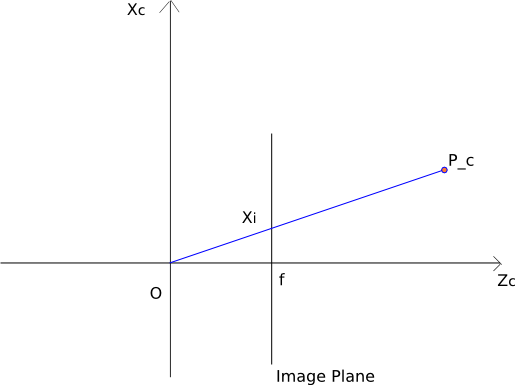
\includegraphics[width=0.7\textwidth]{pics/pinhole_model2}
		\caption{Pinhole Camera Model}
		\label{fig:ch1-pinhole}
	\end{figure}
			
	As seen from Figure \ref{fig:ch1-pinhole} the image plane is located a distance $f$ from the image plane. 
	The point is projected through the hole an onto the image plane. The principal axis of the camere is located in the
	direction of the observed point. For simplicity the image plane are located in the front of the
	pinhole, this is just in theory and is not possible in real camera application. From this the
	perspective equations are derived. \cite{robotbok}
	\begin{equation}
		\label{eq:ch1-perspective}
		P_i = \left[ \begin{array}{cc}
					\frac{f}{z_c} & 0 \\
					0	& \frac{f}{z_c} 
				\end{array} \right] 
				\left[ \begin{array}{c}
					x_c \\
					y_c
					\end{array} \right]
	\end{equation}
	This are the perspective equations which gives the observed point in screen cooridnates. 

\section{Kalman filter}
	Kalman filtering a powerful and versatile tool in estimation and sensor fusion. A Kalman filter is
	usually employd in navigation applications to fuse GPS and INS together. By this way one will have
	the speed and resolution of an INS system and the precission of the GPS system.
	

	The Kalman Filter is as stated befor a very versatile tool which can be employed allmost in
	any application. The downside with the Kalman filter is that it is a Linear system, and can only
	guarantee optimality for linear systems. The system considered in this report is nonlinear and one can not
	use the Kalman filter directly on this system. There is a nonlinear version of the Kalman filter, the
	Extended Kalman Filter, which uses the same assumptions as the linear version but uses the nonlinear
	model to predict the state forward. When updating the Covariance matrix the system equations are
	linearized around the current estimate and updated according to certain update laws. This introduces some
	significant problems. First the filter might converge towards wrong values, because of a non-positive-definite
	covariance matrix. This is mostly due to poor linearization of the state equations. \cite{kalman}
	
\section{Guidance Algorithms}
        \label{chap1-guidance-alg}
        The guidance algorithm is one of the most important part of an autonomous vehicles control system. It
	needs to be robust and be able to handle moast situations. A guidance system should be able to give
	feasible commands to the lower level control system which controls the actuators, and should be able
	to handle most situations with care. The guidance system should decide the best trajectory to be
	followed based on the target location and physical capabilities of the system.\cite{GuidanceReview}

	Most of the guidance algorithms originates from airborne missile systems. This have been well
	documented and proven to work in numerous cases. Common guidance scheems such as Line-of-sight (LOS)
	and Proportional Navigation Guidance (PNG) and vareious implementations of these are employed in
	numerous guidance systems.
	
		\begin{figure}[hbtp]
		\centering
		\includegraphics[width=0.83\textwidth]{pics/waypoint}
		\caption{Variables assosiated with path following}
		\label{fig:ch2-pathfollowing}
	\end{figure}
	The Figure \ref{fig:ch2-pathfollowing} shows the variables which are important for linear path following. The
	cross-track error, $e$ are an important aspect here. It is the lateral position error decomposed in
	the desired path reference frame. Another variable worth noting is $\Delta$ which is the look-ahead
	distance. This is analogus to when you drive a car you look farther down the road to better maneuver
	the car. A great look-ahead distance yealds smooth heading reference but slower convergence of the
	cross-track error. A lower look-ahead distance gives an agressive heading reference and fast
	convergence of the cross-track error. The $s$-variable are called the along-track distance from point
	$P_k$. 
	
	
	\subsection{Line-of-Sight Guidance Law}
	        Line-of-sight-guidance are the most common principle used. The LOS-algorithm computes
		the line-of-sight angle from the present location to the target location, and uses this
		angle as a reference heading.

		The LOS-angle is fed directly into the 
		heading controller as a reference. When ocean currents and disturbances are present, a
		modified guidance law is presented. This uses the Side Slip angle, defined as:
		\begin{equation}
			\label{eq:ch2-sideslip}
			\beta = \sin^{-1} ( \frac{v}{\sqrt{u^2 + v^2 + w^2}})
		\end{equation}
		The new heading reference is then taken as
		\begin{equation}
			\label{eq:ch2-los-law}
			\psi_d = \psi_{LOS} - \beta
		\end{equation}
		Where $\psi_{LOS}$ is the LOS-angle from the current position to the next waypoint. 

	\subsection{Radius-based Guidance}
		Radius-based guidance uses the point where the radius around the current location intersects
		with the path, denoted on Figure \ref{fig:ch2-pathfollowing} as $P_{int}$. This
		means assigning the desired heading as 
		\begin{equation}
			\psi_d = \tan^{-1}(\frac{y_{int} - y}{x_{int} - y})
		\end{equation}
		where 
		\begin{equation}
			(x_{int} - x)^2 + (y_{int} - y)^2 = r^2
		\end{equation}
		If $r$ is chosen sufficiently large the equations above will have a solution, i.e $r > |e|$
		otherwise there will exist no intersection point on the track line.
		\cite{guidance_planar_path}
	
	\subsection{Lookahead-based Guidance}
		Here the lookahead distance are utilized when calculating the desired heading. If $\psi_d$ are
		chosen as:
		\begin{equation}
			\psi_d = \alpha_k + \psi_r
		\end{equation}
		where $\alpha_k$ is the angle of the path and
		\begin{equation}
			\psi_r = \tan^{-1} (\frac{-e}{\Delta})
		\end{equation}
		By choosing $\psi_r$ in this way the heading is always directed towards the lookahead point at
		the path. It is then easily seen that the cross-track error will converge to zero. This
		method is easier and less computationally intensive than the previously stated Radius-based
		guidance. \cite{guidance_planar_path}

		This method are implemented in the guidance system, because of it simplicity and robustness.
		This method are chosen because pipelines are mostly made up of linear segments. 

	
	\subsection{Proportional Navigation}
		Proportional Navigation Guidance is more effective that LOS-guidance in case of a
		non-maneuvering
		target. It gives less interception time than LOS. The PNG-law can be stated as the following:
		\cite{GuidanceReview}
		\begin{equation}
			\eta_c = N' V_c \dot{\lambda}
		\end{equation}
		where $\eta_c$ is the acceleration command, $N'$ is the navigation ratio, $V_c$ is the closing
		velocity, and $\dot{\lambda}$ is the line of sight angular velocity. The navigation ratio is a
		tuning
		parameter which will give higher demanded acceleration and therby reacing the target in less
		time.

        	The guidance laws mentioned above does not work so well with maneuvering targets and lots of
		solutions have been proposed to make these laws more effective when dealing with moving
		targets. In this case the targets will be non-moving waypoints and the maneuvering laws
		will not be discussed here.
	
	
	\subsection{Various Guidance Concepts}
		A unified path following controller are derived in \cite{control-concept-AUV}. The 
		authors proposes a singel control structure which will work for the entire velocity regiem.
		The controller is derived using backstepping. The concept are shown to be Uniform Global
		Expontially Stable under some assumptions about the guidance signals. The controller will not
		work without properly generated references. The AUV concidered here are fully actuated for low
		speeds but becomes undeactuated for higher speeds. The controller guarantees that the AUV
		converges towards the desired path regardless of if it is underactuated or fully actuated.
		
		In \cite{optimal-cross-track} an optimal cross-track guidance scheme are proposed. It seeks to minimize
		the crosstrack-error, depth, pitch and yaw by using the pitch rate and yaw rate, this is called Model
		Predictive Guidance. Damping and can be added to reduce the commanded pitch and yaw rates which can
		cause overshoot. The guidance scheme are compared against a LOS guidance system and gives good
		results.

	
\section{Different Methods for Pipeline Following Discussed in Literture}
	A literature study was performed to see what other people have acomplished on the subject on AUV and 
	pipeline following. 

	\cite{piscis} describes breefly a prototype AUV equipped with a camera and sonar to carry out pipeline
	inspection missions. The AUV uses controllers for heading, speed and depth and visual guidance to
	follow the pipeline. 
	
	\cite{GuidanceReview} proposes a 2-stage guidance problem. When submerging and ascending to the surface, 
	the AUV uses a LOS guidance law at full speed. When the pipeline is aqcuired the guidacen law is switched 
	to a visual guidance scheem, which allows for a precise guidance over the subsea cable or pipeline. 
		
	In \cite{MPC_pure_pursuit} a guidance system using Model Predictive Control (MPC) and PNG law was used to make 
	a guidance system able to track cables and pipelines on the sea bed using Doppler Velocity Log and Electro-
	Magnetic sensors to find the cable/pipeline. The report utilizes the pure pursuit scheeme, similiar to what 
	predadtors do when they are hunting the pray. The cable/pipeline and AUV is formulated as moving points with 
	mass. The engages in a tail chase with the pipeline ``point``, but the AUV never catches up with it. This 
	method is robust to model uncertanties and handles constraints of the vessel in a systematic way. The controller
	however shows problems when a current is introduced in the system. The AUV drifts of the pipeline, but catches 
	up with the waypoints in the end.
	
	In \cite{Visual_inpsection_of_seabottom_by_AUV} a visual guidance system for inspection of undewater structures 
	is presented. The visual system uses an Extended Kalman Filter to smooth and predict where the structure i.e. 
	pipeline will move in the next sample interval of for the image processing software. A 3 dimentional model 
	of the scene is constructed which then allows the guidance sytem to calculate an input to the controllers.
	
	\cite{reactive_control_AUV} proposes a reactive control approach to pipeline tracking together with a 
	profiling sonar. Reactive control originated from the field of obstacle avoidance in autonomous land and air 
	vehicles. It uses \textit{Deformed Virtual Zones} (DVZ) which describes the interaction between the AUV and 
	the pipeline. The controller tries to minimize the defromation of the DVZ and calculates a feasible control input. 
	The DVZ in this case is a prism with a cylidrical cavity directly underneth the AUV. If the AUV moves away from 
	the pipeline the DVZ will be deformed and the controller will try to counteract the motion. This is a 
	computational inexpensive way of achieving a good pipeline following. This method shows promising results 
	but has yet to be implemented and tested in real-life scenarios. 
	
	In \cite{fuel_optimal_control} a fuel-optimal tracking controller is derived to minimalize the fuel consumption 
	of the AUV. It uses the fact that the least fuel consuming path is the shortest one. This
	paper deives a fuel optimal controller using the estimated fuel consumption as a minimization index. 

	\cite{side_scan_sonar} describes two technices for detecting and tracking pipelines using Side Scan
	Sonar and Multi-Beam Echosounders. Prior knowledge about the pipeline are utilized for the recognision
	of the pipeline. A pipeline creates very distinct shadows in a side scan sonar image and are easy to
	separate from the sea bottom.



\chapter{Modelling}

\section{Problem Formulation}
\label{chap2:problem}
	To solve the pipeline following problem it is important to have a clear and distinct problem formulation. 
	The case where the AUV is guided towards the pipeline is not so much of an interrest because it is a stright 
	forward problem which are the subject of many articles. 

	***WARNING, Usammenhengende*** b�r flyttes

	The following assumptions are needed to define the guidance problem:
		\begin{enumerate}
			\item The pipeline is layed on the sea bottom, which gives the pipeline the same
			height signature as the sea bottom. The guidance problem is then reduced to a
			two-dimentional problem.
			\item The pipeline is modelled as a point in space with a specific velocity which
			moves in the direction of the pipeline.
		\end{enumerate}

	The interresting case is when the AUV is to acquire the pipeline and track it by the means of a camera. The
	camera will output three points, distorted by noise. Since the AUV preferebly will travel with the
	pipeline, the coordinates of interrest will be the y-coordinates of the different points. It would be
	a good ideeg �l gjennom offentlig omr�de er jo en vederstyggelighet,  
	men styret er vel ikke dto formulate the points as points on the pipeline with a velocity moving with the AUV.

	This gives rise to formulate the pipeline as a point moving ahead of the AUV. The vessel will pursue
	this but it is convenient that it will never catch up with it.


\section{AUV model}
	The model used is the one from \cite{fossen}, and is written in the previous chapter, equation \eqref{eq:chp1-model}.
	
	\subsection{Assumptions}
	Assumtions that where made to simplify the modelling and implementation of the AUV system.
		\subsubsection{Low-speed assumption}
		The speed regieme of \textit{HUGIN 1000} is about 1-3 $m/s$. The design speed is around 2 $m/s$. 
		Then the assumtion about low-speed should be adequate.  

		This is a good idea to check. Run a simulation in simulink with the low speed model and the 
		nonlinear model and compare. Discuss later in the report, maybe.
		
		\subsubsection{Measurements}
		The vessel should have enough instrumentation available to measure $\eta$, $\nu$, and $\dot{\nu}$. 
		The distance to the sea bottom should also be available. All this instrumentation is common to 
		include in an standar AUV instrumentation package. 


\section{Camera modelling}
	The camera is modeled using a pinhole camera model. It assumes that the lense is an infintiesmall hole which 
	all light passes through. The image plane is located in the front of the projection plane at a distance $f$, 
	which is called the focus distance. This is not possible in real life, but simplyfies the mathematics a little. 
	This model is used to derive the interaction matrix, $\interaction$, which describes the movement of the 
	points in the image plane to the movement of the camera.\cite{robotbok} 

	The solution of equation \eqref{eq:ch1-image_point_veloc} gives the position of the points relative
	to the AUV. The x-axis of the camera coordinate system is defined along the pipeline, while the y-axis 
	is defined toward the left of the pipeline. This means that the points are moving out of the camera
	field-of-view after a short time, given non-zero \textit{surge}-velocity. Since the goal is to follow
	the pipeline and not a single point, it is convenient to formulate the pipeline as a point moving with
	the AUV with equal velocities. 

	


\section{Pipeline representation}
	In the simulations the pipelines are represented as interpolated waypoints. Waypoint on where the pipeline are
	going is supplied by the user and interpolated using the \textit{matlab}-function \textit{pchip}. 



\section{Kalman filter}
	The Kalman filter is designed with the purpose to smooth the output from the camera, estimate the trajectory 
	of the pipeline if it is lost, and estimate the current forces and moments which is acting on the vessel. 
	The bias is modelled as a \textit{1st order Markov}-model.
	\begin{equation}
		\label{eq:chp2-biasmodel}
		\dot{\mathbf{b}} = -\mathbf{T}^{-1} \mathbf{b} + \mathbf{w} \quad \mathbf{b}, \mathbf{w} \in \mathbb{R}^6
	\end{equation}
	where $\mathbf{w}$ is zero-mean guassian distributed white noise, and $\mathbf{T}$ is a diagonal matrix with 
	large time constants, to model the slowly varying current forces. 
	Equation \eqref{eq:chp2-biasmodel} is restructured by inserting the kinetics equation from the model and gives:
	\begin{equation}
		\dot{\mathbf{b}} = -\mathbf{T}^{-1} \rotation (\restoring) - \mathbf{T}^{-1} 
		\rotation (\mass - \tau + \damping) + \mathbf{w}
	\end{equation}

	
	The state used in the Kalman filter model is $\mathbf{x} = [\mathbf{\eta}^T \quad x_i^T 
	\quad \mathbf{b}^T]^T$, $\mathbf{x} \in \mathbb{R}^{18}$. The velocity vector, $\mathbf{\nu}$, 
	the acceleration, $\dot{\mathbf{\nu}}$, and the forces and moments from the regulator, $\mathbf{\tau}$ is 
	used as input to drive the filter, $\mathbf{u} = [\tau^T \quad \mathbf{\nu}^T \quad \mathbf{\dot{\nu}}^T]^T$. 
	The systems measurement is the position, $\mathbf{\eta}$ and the camera output, $x_i$. The measurement is 
	assumed affected by gaussian distributed white noise, with zero-mean.
	
	The mathematical model used for the Kalman filter is summarized here:
		\begin{align}
			\mathbf{\dot{x}} &= \mathbf{f(x)} + \mathbf{B(x, u) u} + \mathbf{E w} \\
			\mathbf{y} &= \mathbf{H x} + \mathbf{v}
		\end{align}
	where
		\begin{align}
			\mathbf{f(x)} &= \left[ \begin{array}{c}
						\mathbf{0}\\
						\mathbf{0}\\
						-\mathbf{T}^{-1} \rotation \restoring
						\end{array} \right] \quad 
			\mathbf{E} = \left[ \begin{array}{cc}
			                      	\mathbf{0} & \mathbf{0} \\
			                      	\mathbf{I} & \mathbf{0}\\
			                      	\mathbf{0} & \mathbf{I}
			                     \end{array} \right] \quad
			\mathbf{H} = \left[ \begin{array}{ccc}
			                      	\mathbf{I} & \mathbf{0} & \mathbf{0}\\
			                      	\mathbf{0} & \mathbf{I} & \mathbf{0}
			                     \end{array} \right] \\
			\mathbf{B(x, u)} &= \left[ \begin{array}{ccc}
			                      	\mathbf{0} & \rotation & \mathbf{0}\\
			                      	\mathbf{0} & \interaction & \mathbf{0}\\
			                      	\mathbf{T}^{-1} & -\mathbf{T}^{-1}\rotation \mathbf{D(\nu)} 
						& -\mathbf{T}^{-1} \rotation \mathbf{M}
			                     \end{array} \right] &
		\end{align}

	The equations used for the Extended Kalman Filter can be found in \cite{fossen} p199.
	
\section{Controller Design}
	The control system which supply the lower-level control system with forces and moments references, is 
	divided into 3 sub systems:
		\begin{itemize}
		 \item Speed control
		 \item Depth control
		 \item Heading control
		\end{itemize}
	This is called the flightmode controller, which is used for normal pipeline tracking, descent and ascent. 
	
	A fine-positioning controller is used to position the AUV on top of the pipeline and keep it there regadless 
	of ocean currents. This is to provide good pictures for the pipeline inspection mission.
	
	The \textit{HUGIN 1000} is a sleender-body type AUV. The coupling effects in in the surge and sway can be 
	neglected, and therfor decoupled. This means that one can create two subsystems from the AUV model: 
	The \textit{surge} subsystem, and the \textit{sway-yaw} subsystem. 
	
	TODO: Lage en figur som viser hvordan kontrollsystemet er bygget opp.
	
	TODO:Too keep the AUV right on top of the pipeline one can use kinematic control to with feedback from the 
	camera too keep the AUV right on top of the pipeline using theory from robot control by visual means.
	
	
	TODO:********Utledning og stabilitetsbevis for alle kontrollerene*******
	\subsection{Speed Controller}
		The speed controller is derived form the \textit{surge}-subsystem, called \textit{surge}-model
		\cite{fossen}. Under the slow speed assumption, the coriolis/centripetal-matrix is assumed
		zero, $\coriolis \approx 0$  
		\begin{equation}
			(m - X_{\dot{u}})\dot{u} - X_u u - X_{|u|u}|u| u = \tau_1
		\end{equation}
	
	
	
	\subsection{Depth Controller}
		To derive the depth controller in the crusing control system the
		\textit{longitudinal}-subsystem is used as the control model.

	
	\subsection{Heading Controller}
		Using the \textit{lateral}-subsystem representation from \cite{fossen}. Under the assumtions
		that $u, w, p, q, r, \phi,$ and $\theta$ from the longitudinal subsyustem are small, the
		kinematics are reduced to:
		\begin{align}
			\dot{\phi} &= p \\
			\dot{\psi} &= r 
		\end{align}
		The low-speed assumtions is utilized and higher order velocity terms are neglected, and
		constant \textit{surge}-velocity are assumed. This gives the following system:
		\begin{equation}
			\begin{aligned}
				\left [ \begin{array}{ccc}
					m - Y_{\dot{v}} & - m z_g - Y_{\dot{p}} & m x_g - Y_{\dot{r}} \\
					-m z_g - Y_{\dot{p}} & I_x - K_{\dot{p}} & I_{zx} - K_{\dot{r}} \\
					m x_g - Y_{\dot{r}} & I_{zg} - K_{\dot{r}} & I_z - N_{\dot{r}} 
					\end{array} \right]
				\left [ \begin{array}{c}
					\dot{v} \\
					\dot{p} \\
					\dot{r} 
					\end{array} \right] \\
				+ \left [ \begin{array}{ccc}
					-Y_v	&	-Y_p 	&	-Y_r \\
					-M_v	&	-M_p	&	-M_r \\
					-N_v	&	-N_P	&	-N_r
					\end{array} \right]
				\left [ \begin{array}{c}
					v \\
					p \\
					r 
				\end{array} \right] + 
				\left [ \begin{array}{ccc} 
					0 & 0 & (m - X_{\dot{u}})u \\
					0 & 0 &  0 \\
					(X_{\dot{u}} - Y_{\dot{v}}) u & 0 & m x_g u 
					\end{array} \right]	
				\left [ \begin{array}{c}
					v \\
					p \\
					r 
				\end{array} \right] \\
				+  \left [ \begin{array}{c}
					0 \\
					W z_b \sin \phi \\
					0 
					\end{array} \right] = \left [ \begin{array}{c}
									\tau_2 \\
									\tau_4 \\
									\tau_6
								      \end{array} \right ]
			\end{aligned}
		\end{equation}
		The \textit{roll}-state can be removed from the equations because of the assumtions of small
		$\dot{p}, p$. 


	
	\subsection{Over-Pipeline Tracking Controller}
		When the AUV is over the pipeline the need to keep the AUV on top of the pipeline to get deecent 
		pictures for the pipeline inspection, presents itself. To solve this problem a second controller 
		have been created just for this purpose. Since the vessel is controllable in 5 DOF the ability to 
		create a good controller for this purpose is good. 
		
		The controller uses input form the camera to get the position of the AUV relative to the pipeline 
		and give a suitable input to the controller.
		
\section{Guidance system}
	The guidAnce system on the \textit{HUGIN1000} AUV needs to be robust and tolerant to disturbances. The 
	vessel will be operating in the vicinity of ocean currents and other unpredictable factors which have to 
	be countered by the guidance system in a smart and robust way.
	
	
	
	\subsection{Line-of-Sight Guidance Law with Current Compensation}
		This is described in Section \ref{chap1-guidance-alg}. The LOS-angle is fed directly into the 
		heading controller as a reference. When ocean currents and disturbances are present, a modified 
		guidance law is presented. This uses the Side Slip angle, defined as:
		\begin{equation}
			\label{eq:chap2-sideslip}
			\beta = \sin^{-1} ( \frac{v}{\sqrt{u^2 + v^2 + w^2}})
		\end{equation}
		an alternative defenition of the side slip angle:
		\begin{equation*}
			\beta = \tan^{-1} (\frac{v}{u})
		\end{equation*}
		The new heading reference is then taken as
		\begin{equation}
			\label{eq:chap2-los-law}
			\psi_d = \psi_{LOS} - \beta
		\end{equation}
		Where $\psi_{LOS}$ is the LOS-angle from the current position to the next waypoint.
		
		The guidance law \eqref{eq:chap2-los-law} is used in the initial descent from the sea surface to the 
		starting position on the pipeline and final ascent to the surface, and other long-distance guidance.
		
	\subsection{Cross-Track Error Controller}
		The cross-track error is defined as the distance from the vessel to the Line-of-Sight line between 
		two waypoints. This controller seeks to minimize this error. The idea behind this controller is that 
		this should keep the AUV on top of the pipeline in the presence of current.
		
		TODO: Derive the Cross-track error guidance law. \cite{cross-track}
		
		
		
	
\section{Trajectory Generation}
	Do I need trajectory generation? 	
	

\chapter{Simulations and Results}
	\label{ch3}
	To test the performance of the proposed guidance system, it is implemented in matlab/simulink. A number of
	scenarios are used to test how it performes in various conditions.
	

\section{Matlab}
	The mathematical model of the \textit{HUGIN 1000} AUV are implemented in simulink using the
	\textit{GNC} toolbox available from \textit{www.marinecontrol.org} with slight modifications to the
	6DOF model.

	The Camera output simulator were programmed in matlab. It inputs the position of the AUV and
	transforms it to body coordinates to calculate the field of view of the camera. The camera are based
	on the pinhole camera model with unity focus distance, and a view angle of about 45 degrees. The
	program then calculates the field of view of the camera and checks if there are any part of the
	pipeline inside the field of view. The output of the camera are three points taken out at the top, the
	middle and the bottom of the field of view. See Algorithm~\ref{alg:ch3-camsim}
	\begin{algorithm}[htbp]
		\hrule
		\caption{Camera Simulatior($\eta(t)$, $z_b(t)$, $f$)}
		\label{alg:ch3-camsim}
		\hrule
		\hrule\vspace{\onelineskip}
		\begin{algorithmic}
			\STATE FieldOfView $= f(\eta(t), z_b(t), f)$
			\IF{Pipeline inside FieldOfView}
				\STATE{PipelineSegment inside FieldOfView} to image cooridnates
			\ENDIF
			\RETURN{PipelineSegment in image coordinates}
		\end{algorithmic}
		\vspace{\onelineskip}\hrule
		\vspace{0.2pt}
	\end{algorithm}

	A sonar which determines the altitude are implemented using a look-up table with a predefined bottom
	profile.

	The descision logic is implemented as a state machine with three states, and gives out the 
	desired heading dependent on what state the system is in. This implementation is in correspondance
	with  Figure~\ref{fig:ch2-flowdiagram}.

	The filter was created using a m-file and global variables for the filter parameters. The filter
	parameters are as follows:
	\begin{equation*}
		P_0 = \left [ \begin{matrix}
				10 & 0 & 0 & 0 \\
				0 & 10 & 0 & 0 \\
				0 & 0 & 0.1 & 0 \\
				0 & 0 & 0 & 0.1
				\end{matrix} \right] \quad
		W = 0.1 \mathbf{I}_{2x2} \quad Q = 10 \mathbf{I}_{2x2} 
	\end{equation*}
	The $\mathbf{T}$ matrix are chosen to be diagonal with $1000$ at both elements.

	The final simulink diagram are shown in figure \ref{fig:ch3_simulink}.
	\begin{figure}[htbp]
		\centering
		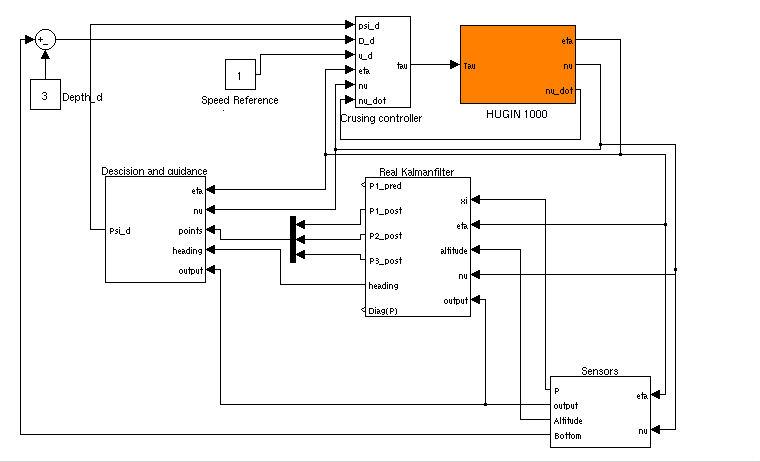
\includegraphics[width=\textwidth]{pics/simulink}
		\caption{The Simulink Diagram of the implemented Guidance System}
		\label{fig:ch3_simulink}
	\end{figure}
	The structure of the model are strictly modular and the blocks shown in the simulink diagram have the
	same function as in Figure~\ref{fig:ch2-blockdiagram}. This allows to update and improve the different
	blocks individually, without designing a new system.

	

\section{Simulation Scenarios}
	To test the performance of the guidance system some scenarios are proposed. In all the scenarios the
	pipeline are located at the sea bottom around 10 meters bellow the surface.The depth is arbitarily
	chosen and the value does change the scenarios except that the submerging time is longer. The AUV 
	will start at the surface and submerge towards the starting point of the pipeline or the mission. 
	\begin{description}
		\item[\textbf{1$^{\mathrm{st}}$ Scenario}.] The pipeline are at the exact location acording 
		to predefined data. Environmental disturbances such as currents are turned off. The pipelien are
		continiously visible for the camera the whole inspection distance. Reference simulation.
		\item[\textbf{2$^{\mathrm{nd}}$ Scenario}.] Exact as over but with environmental forces turned on.
		\item[\textbf{3$^{\mathrm{rd}}$ Scenario}.] The pipeline are at the exact location where 
		it initially was layed. A section is burried, and not visible for the camera. Environmental
		forces are turned on.
		\item[\textbf{4$^{\mathrm{th}}$ Scenario}.] The \'a priori information about the pipeline 
		are offset about 50 meteres to test the ability of the guidance system to search for the pipeline.
	\end{description}


\section{Results}
	The matlab/simulink implementation were simulated with the given setup. A simulation were done to
	check if the low speed assumptions were valid. After this the simulation of the scenarios were done
	and produced the followin results.


	\subsection{Test of the low-speed assumtion}
		In figures \ref{fig:ch3_coriolis_forces} and \ref{fig:ch3_damping_forces} the forces and
		moments created by the Coriolis/centripetal and damping matrices are recorded. In Figure
		\ref{fig:ch3_coriolis_forces} the sway degree of freedom are dominant, and peaking about
		-400N during the turning maneuvers of the AUV. The forces and moments created by the coriolis
		terms are partially counteracted by the damping terms, that also have greated magnitude than
		the coriolis terms.
		\begin{figure}[htbp]
			\centering
			\subfigure[Coriolis Forces]{
				\label{fig:ch3_coriolis_forces}
				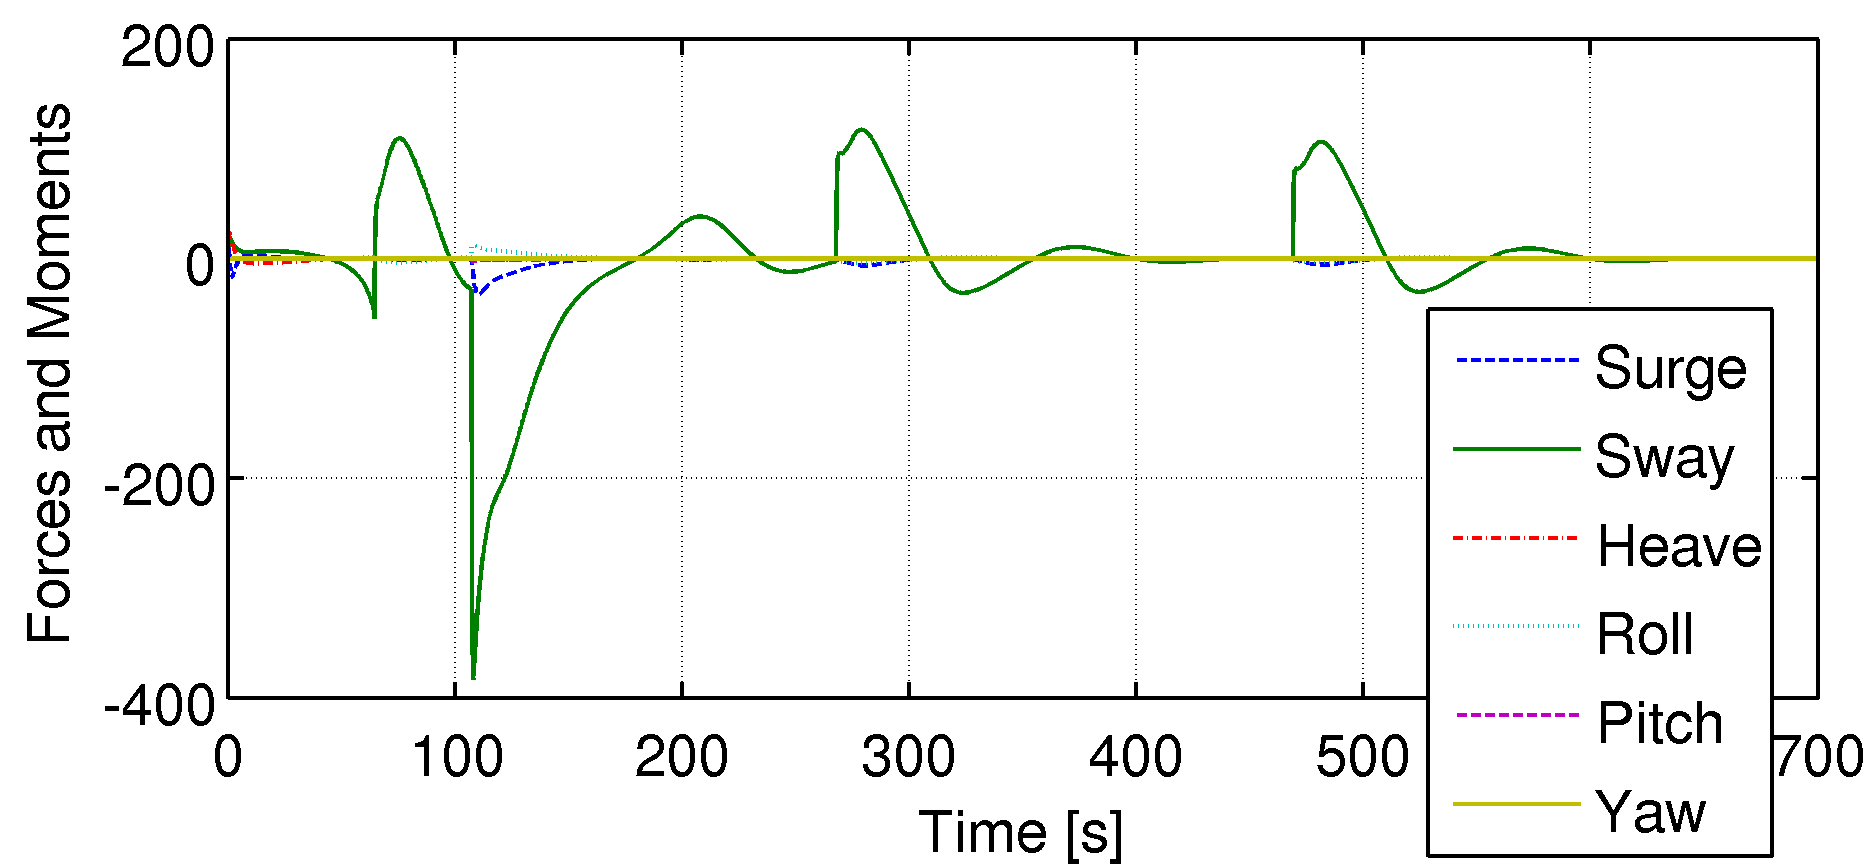
\includegraphics[width=0.7\textwidth]{pics/coriolis_forces}
			}	
			\subfigure[Dampering Forces]{
				\label{fig:ch3_damping_forces}
				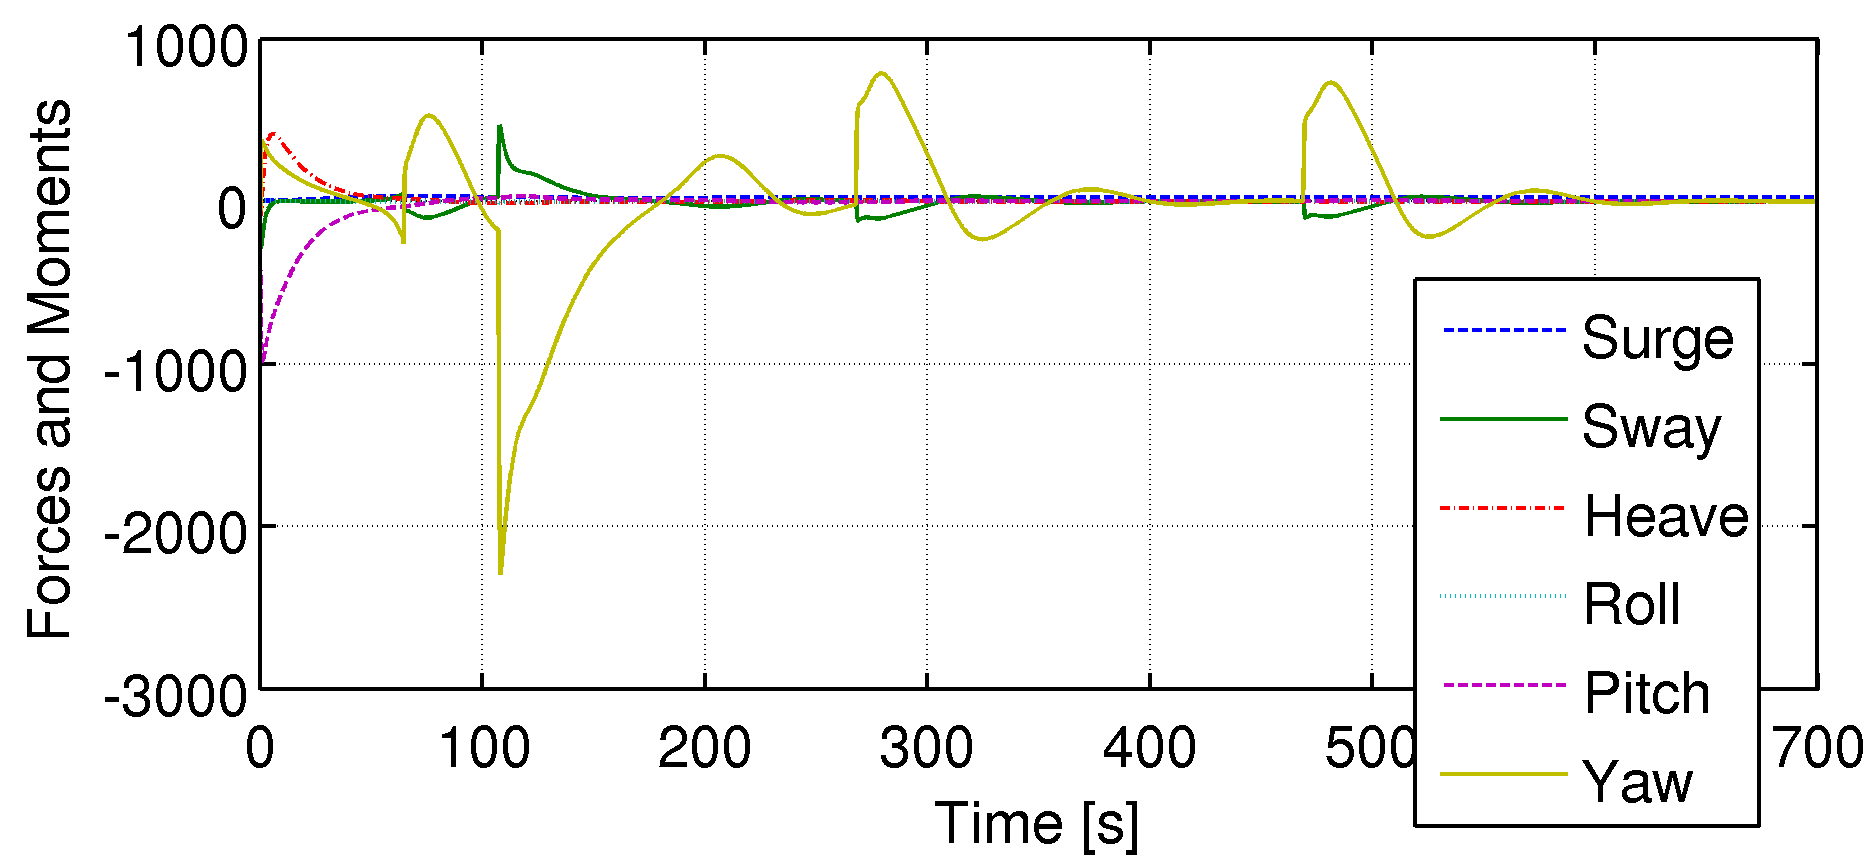
\includegraphics[width=0.7\textwidth]{pics/damping_forces}
			}
			\caption{The Forces associated with the AUV maneuvering}
			\label{fig:ch3-maneuvering forces}
		\end{figure}
		This suggests that the coriolis/centripetal forces can be neglected and compensated for as
		model errors in the controller using integral terms.  

	\subsection{1$^{\mathrm{st}}$ Scenario}
		This is a reference test to see how the guidance system performs on the ideal case.
		To show the sensitivity to the envirionmental disturbances, introduced in later scenraios.
		\begin{figure}[htbp]
			\centering
			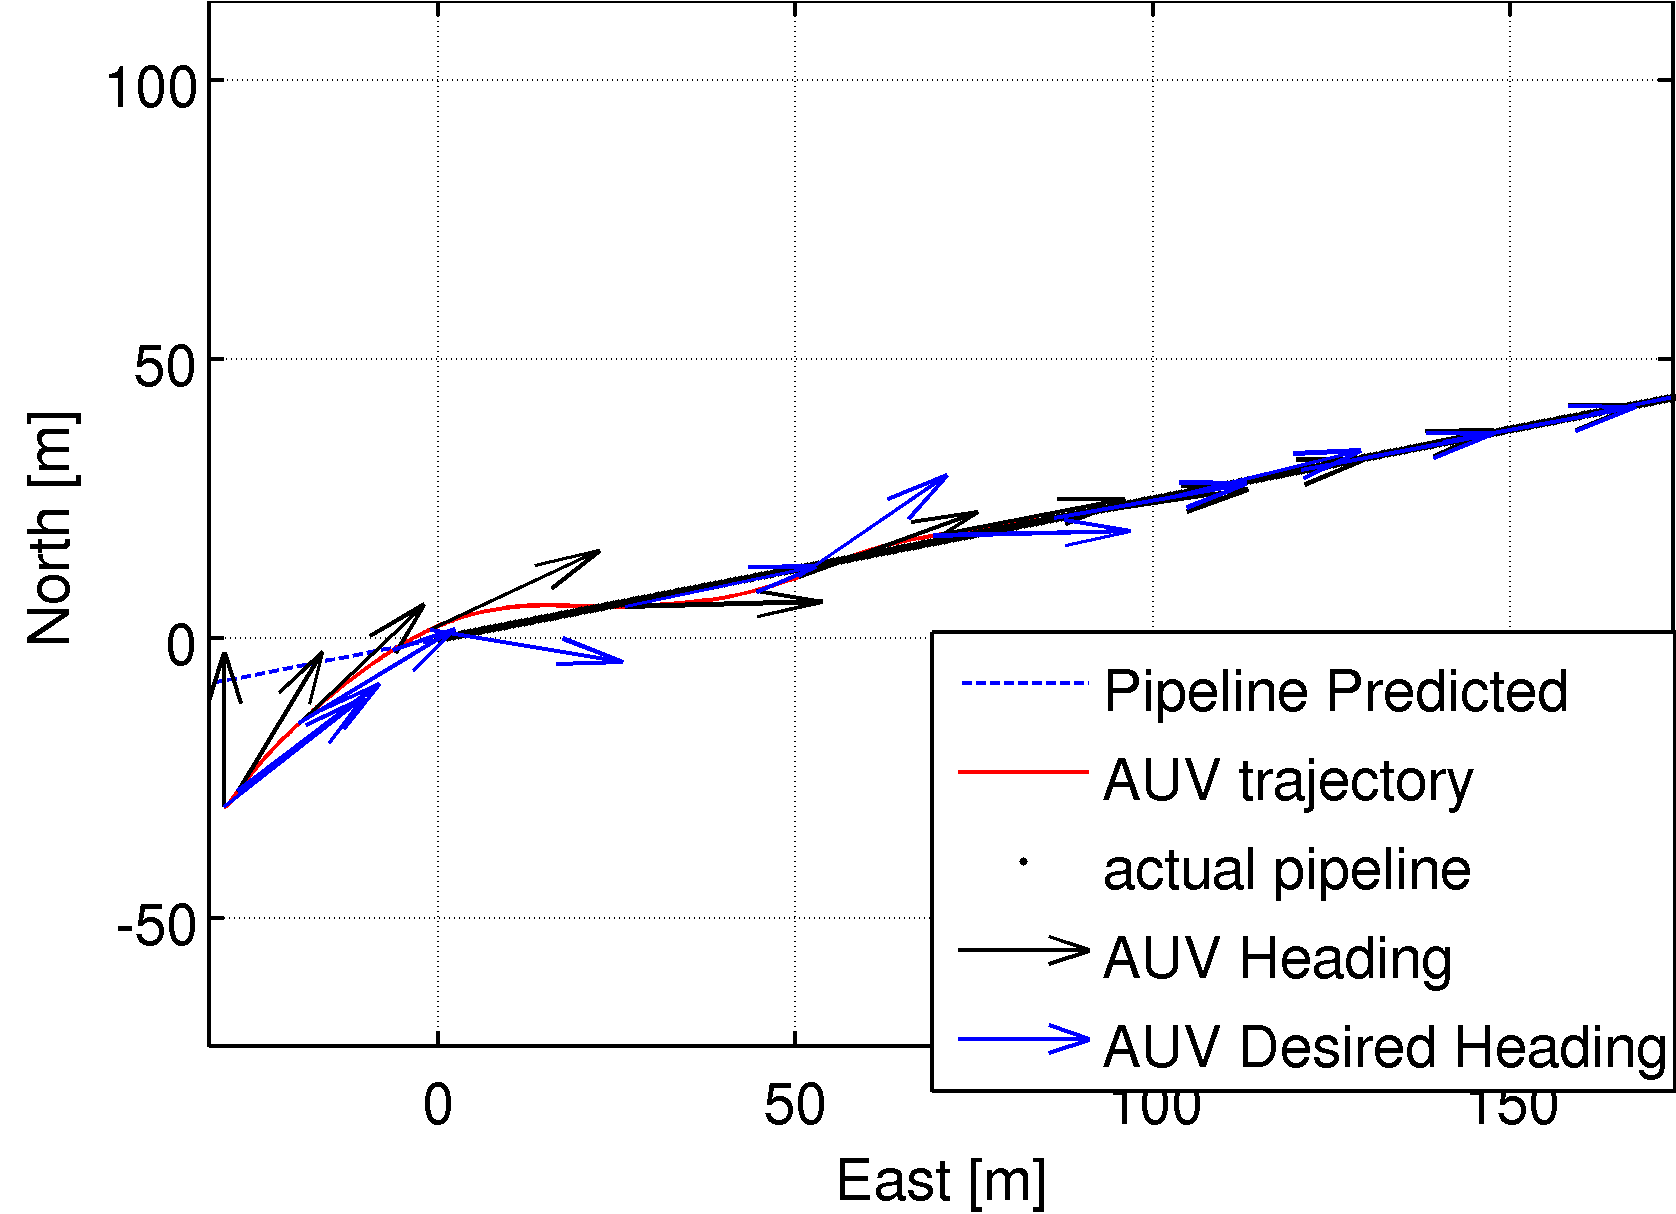
\includegraphics[width=0.7\textwidth]{pics/1st_NE_path}
			\caption{North East path of AUV without Current}
			\label{fig:ch3_1st_NE_path}
		\end{figure}
		\begin{figure}[htbp]
			\centering
			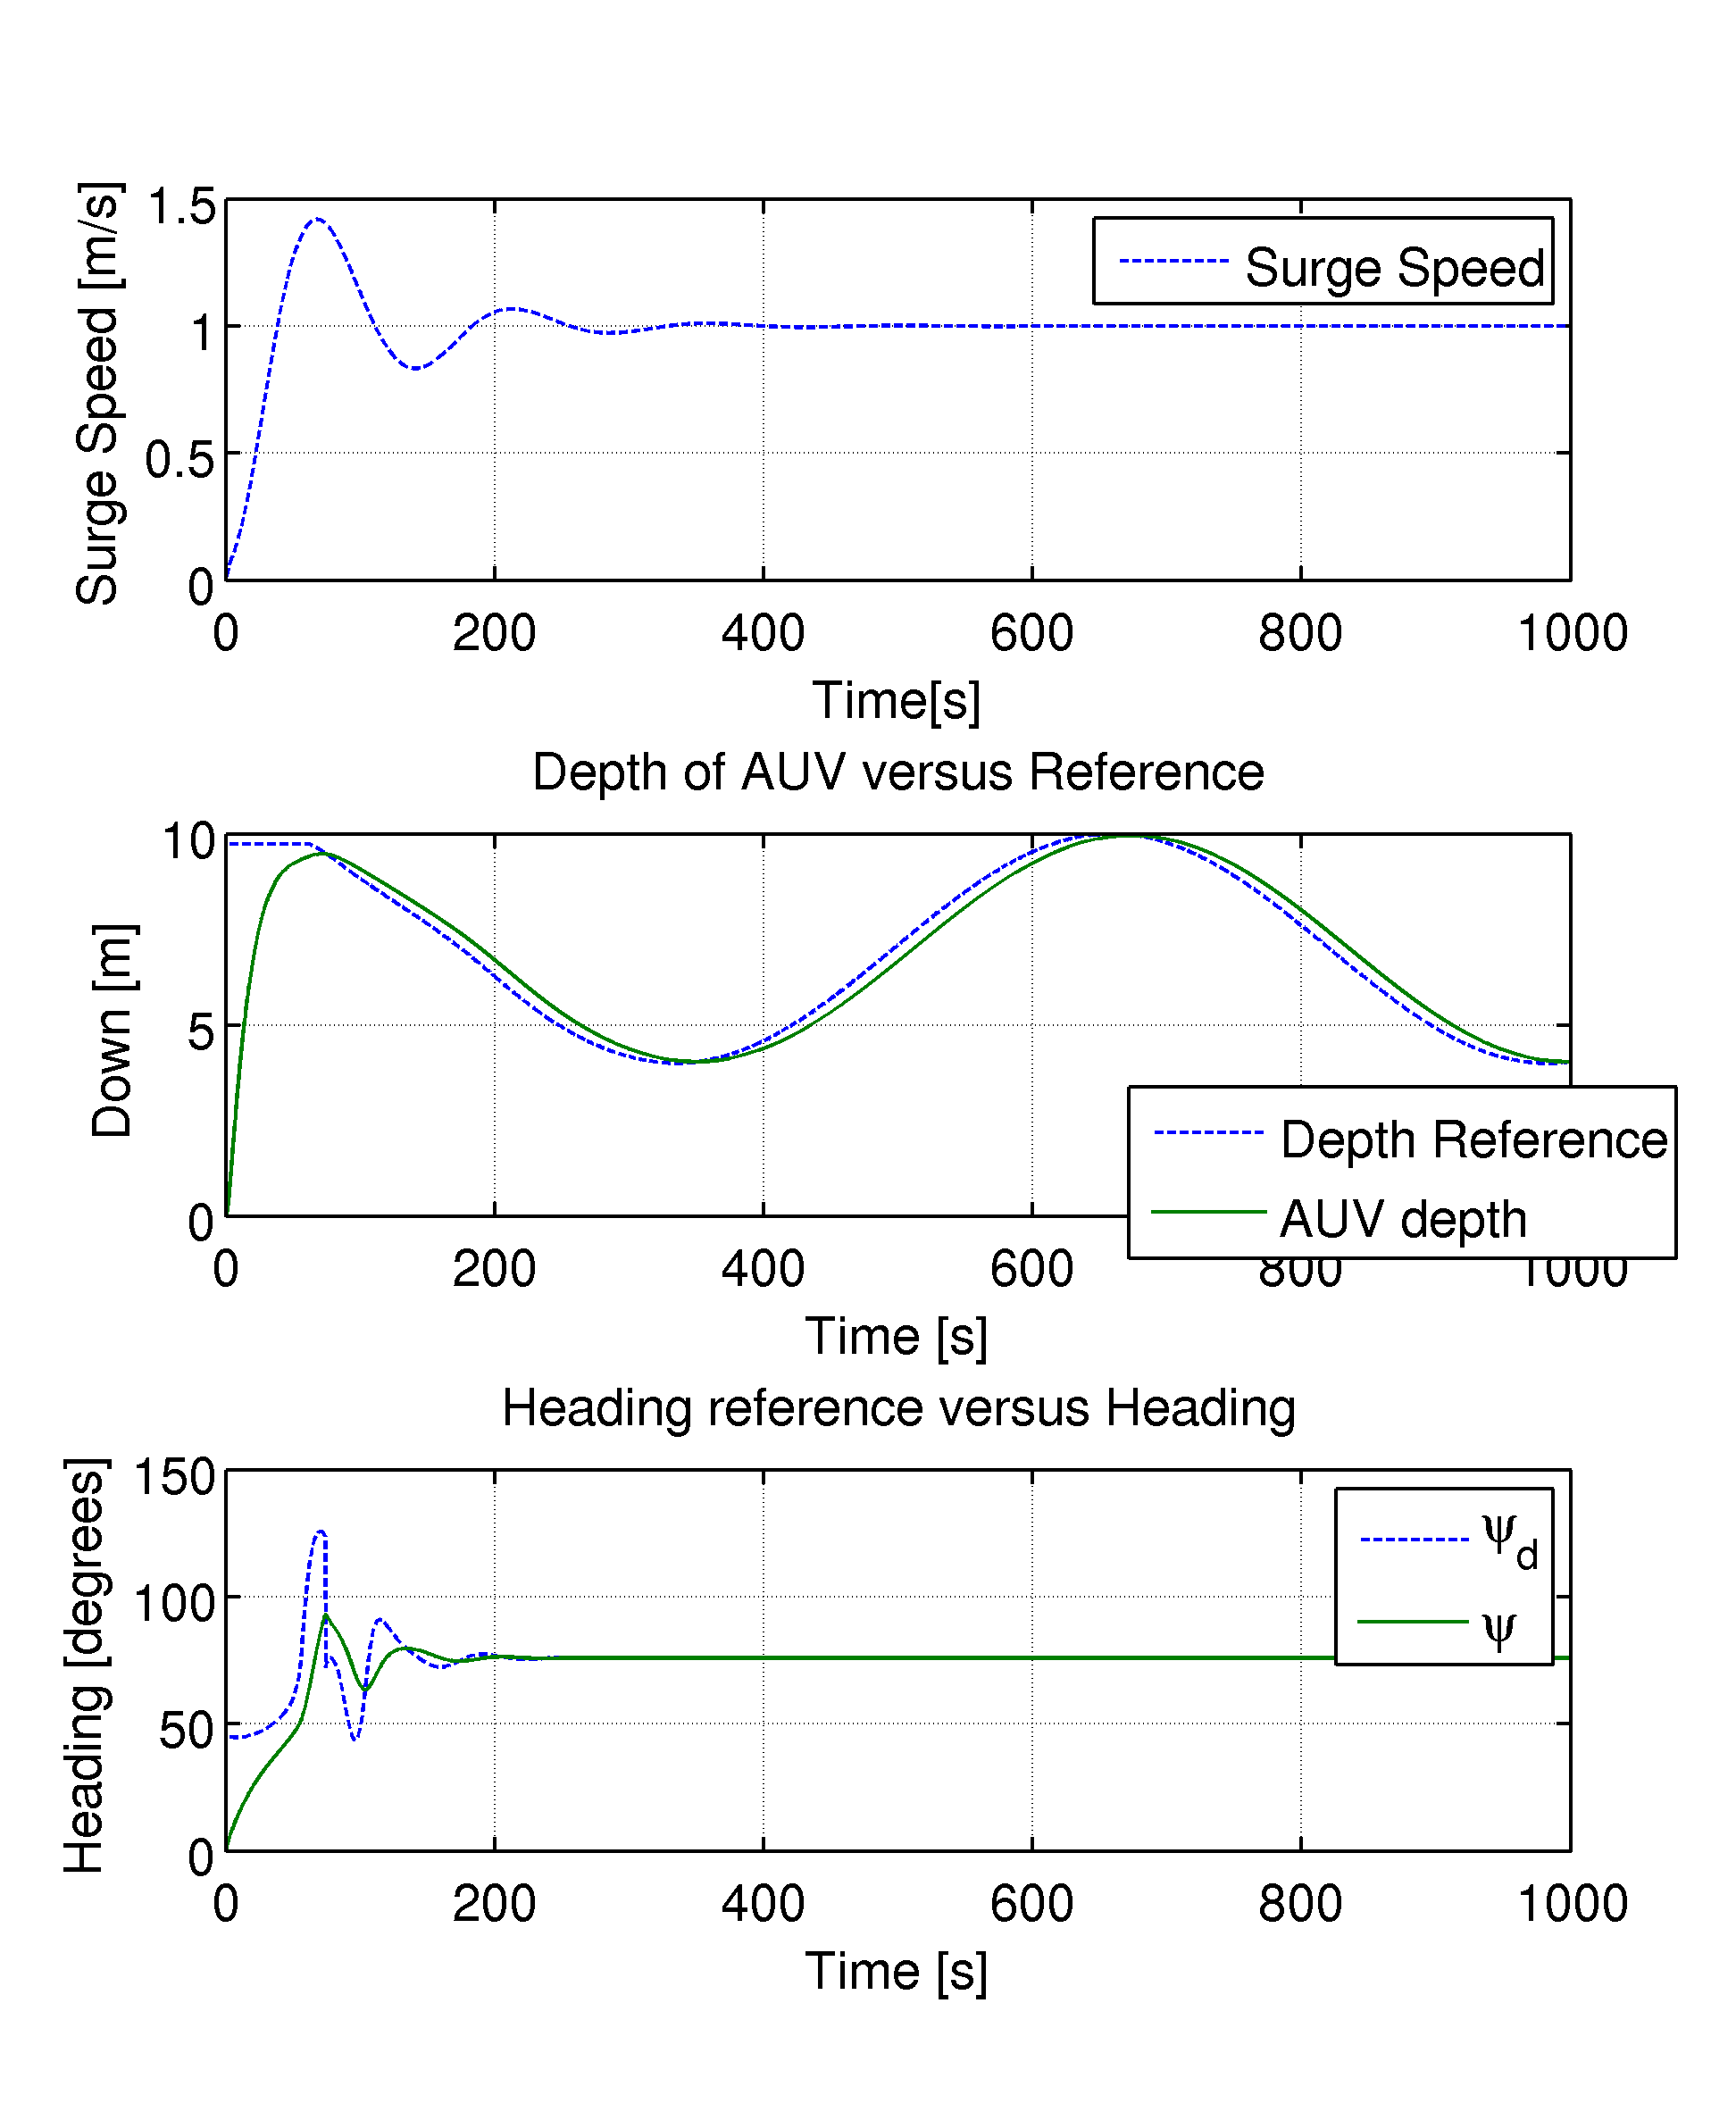
\includegraphics[width=0.75\textwidth]{pics/1st_uDpsi}
			\caption{Surge-, Depth- and Heading- Reference vs. Actual Values}
			\label{fig:ch3_1st_uDpsi}
		\end{figure}
		
		It can be seen from both Fiugre \ref{fig:ch3_1st_NE_path} and the
		third plot on Figure \ref{fig:ch3_1st_uDpsi} that the heading reference, $\psi_d$ have some
		oscilatory nature. This is because of the relatively low look-ahead distance defined in the
		guidance algorithm. This can be analogus to when driving a car and you fix your gaze on
		the road not very far ahead of the car, and you will get more uneasy driving and jerking
		motion. 

		The depth reference are given by the bottom which are constructed using a look-up table
		created by a sinuosidal plane. The reference are followed pretty well. The delay on the
		action by the controller are created because the \textit{heave} direction are not directley
		controlled, but are relayed through the \textit{pitch} degree of freedom. This could probably
		have been reduced by feeding the reference into the controller as well. This will help the
		controller predict the motion and compensate for it when it happens.

		It is worth noting that the \textit{surge} speed overshoots, but is not seen as a problem for
		further simulation and analysis. The overshoot can be removed by including derivative action
		in the Speed controller. This would reduce the commanded force when reaching the set point.

	
	\subsection{2$^{\mathrm{nd}}$ Scenario}
		The environmental forces are now turned. The current is assumed only effective in the North
		East plane and has no effect in the \textit{heave}-direction. The current is moving from
		north-west to south-east, heading $-45^{\circ}$ and have a strength of $0.3$ m/s. 
		
		\begin{figure}[htbp]
			\subfigure[NE Path with	Waypoints]{\label{fig:ch3_2nd_NE_wpt}
				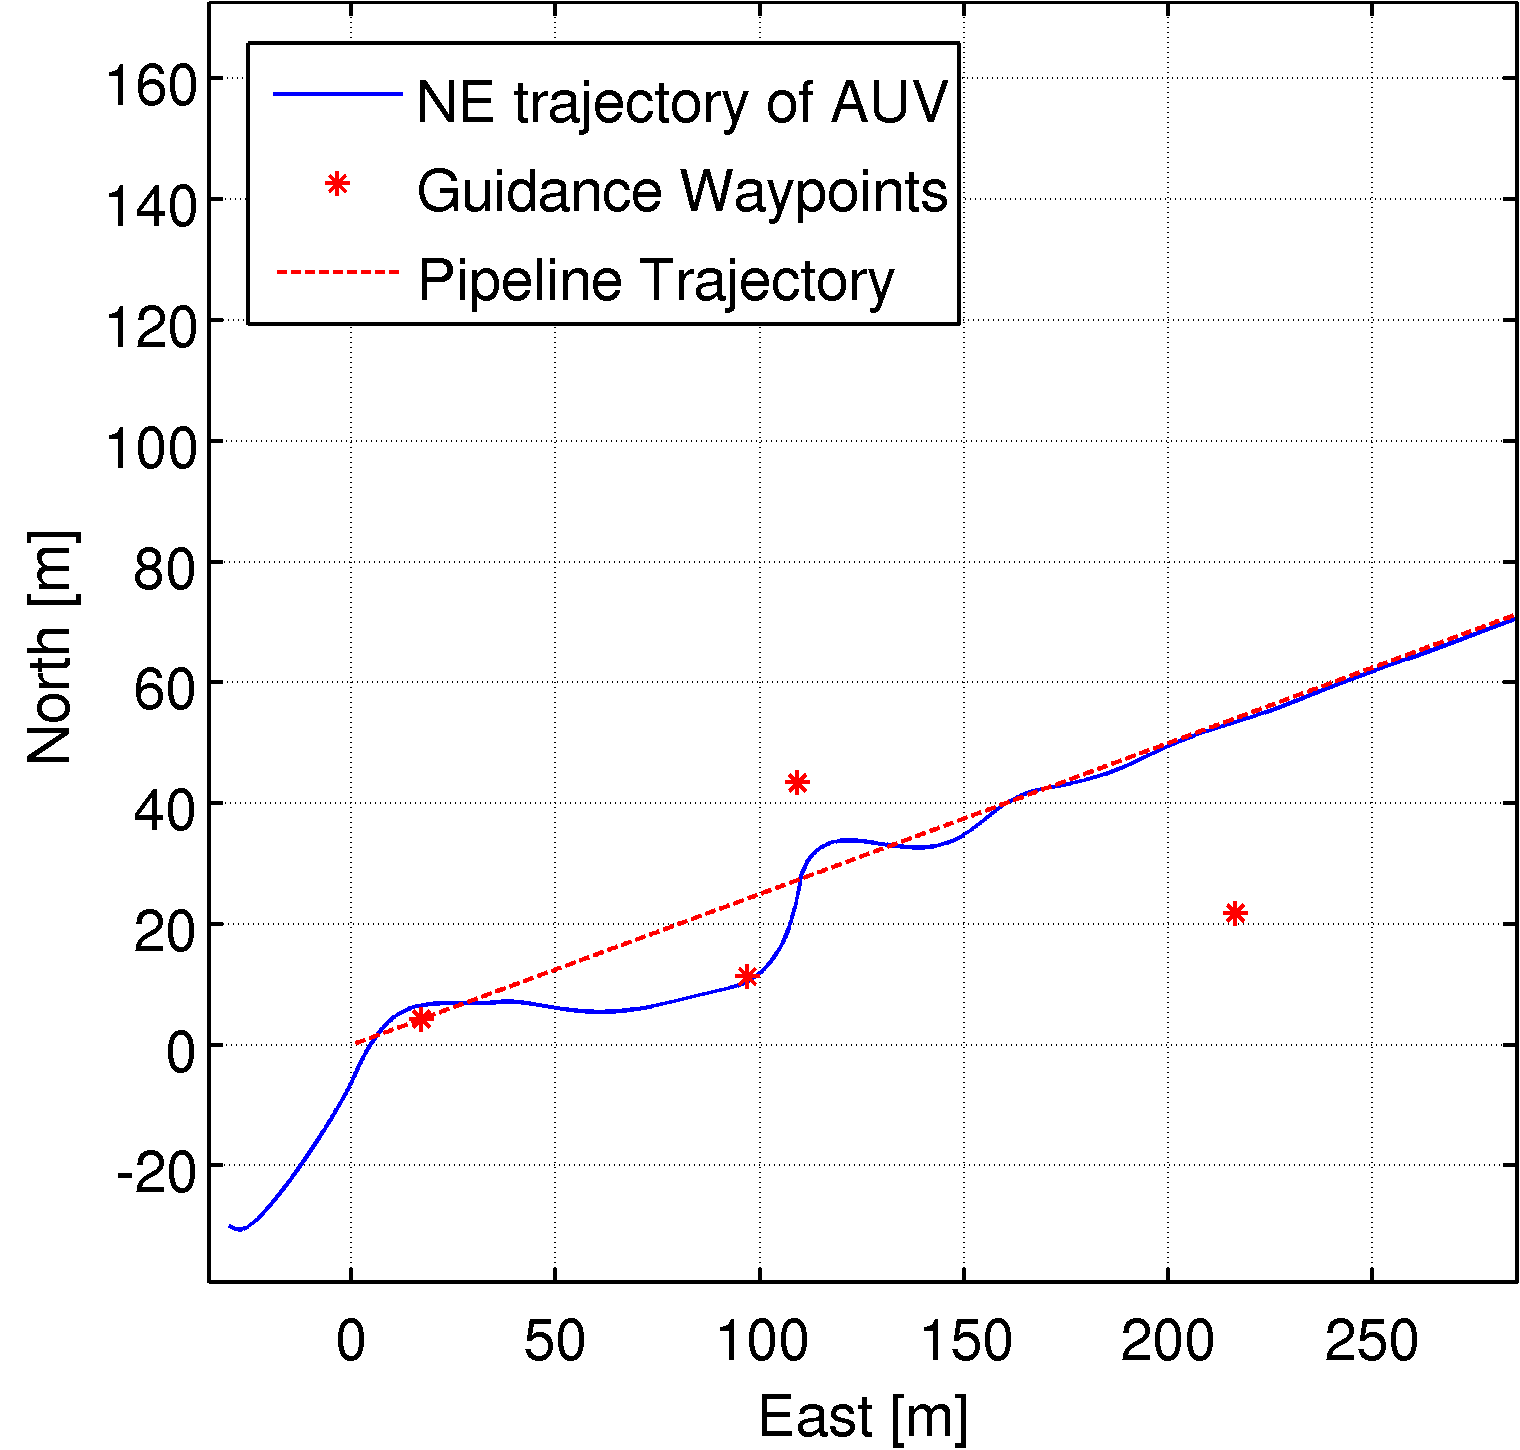
\includegraphics[width=0.5\textwidth]{pics/2nd_NE_wpt}}
			\subfigure[NE path with	Heading]{\label{fig:ch3_2nd_NE_path}
				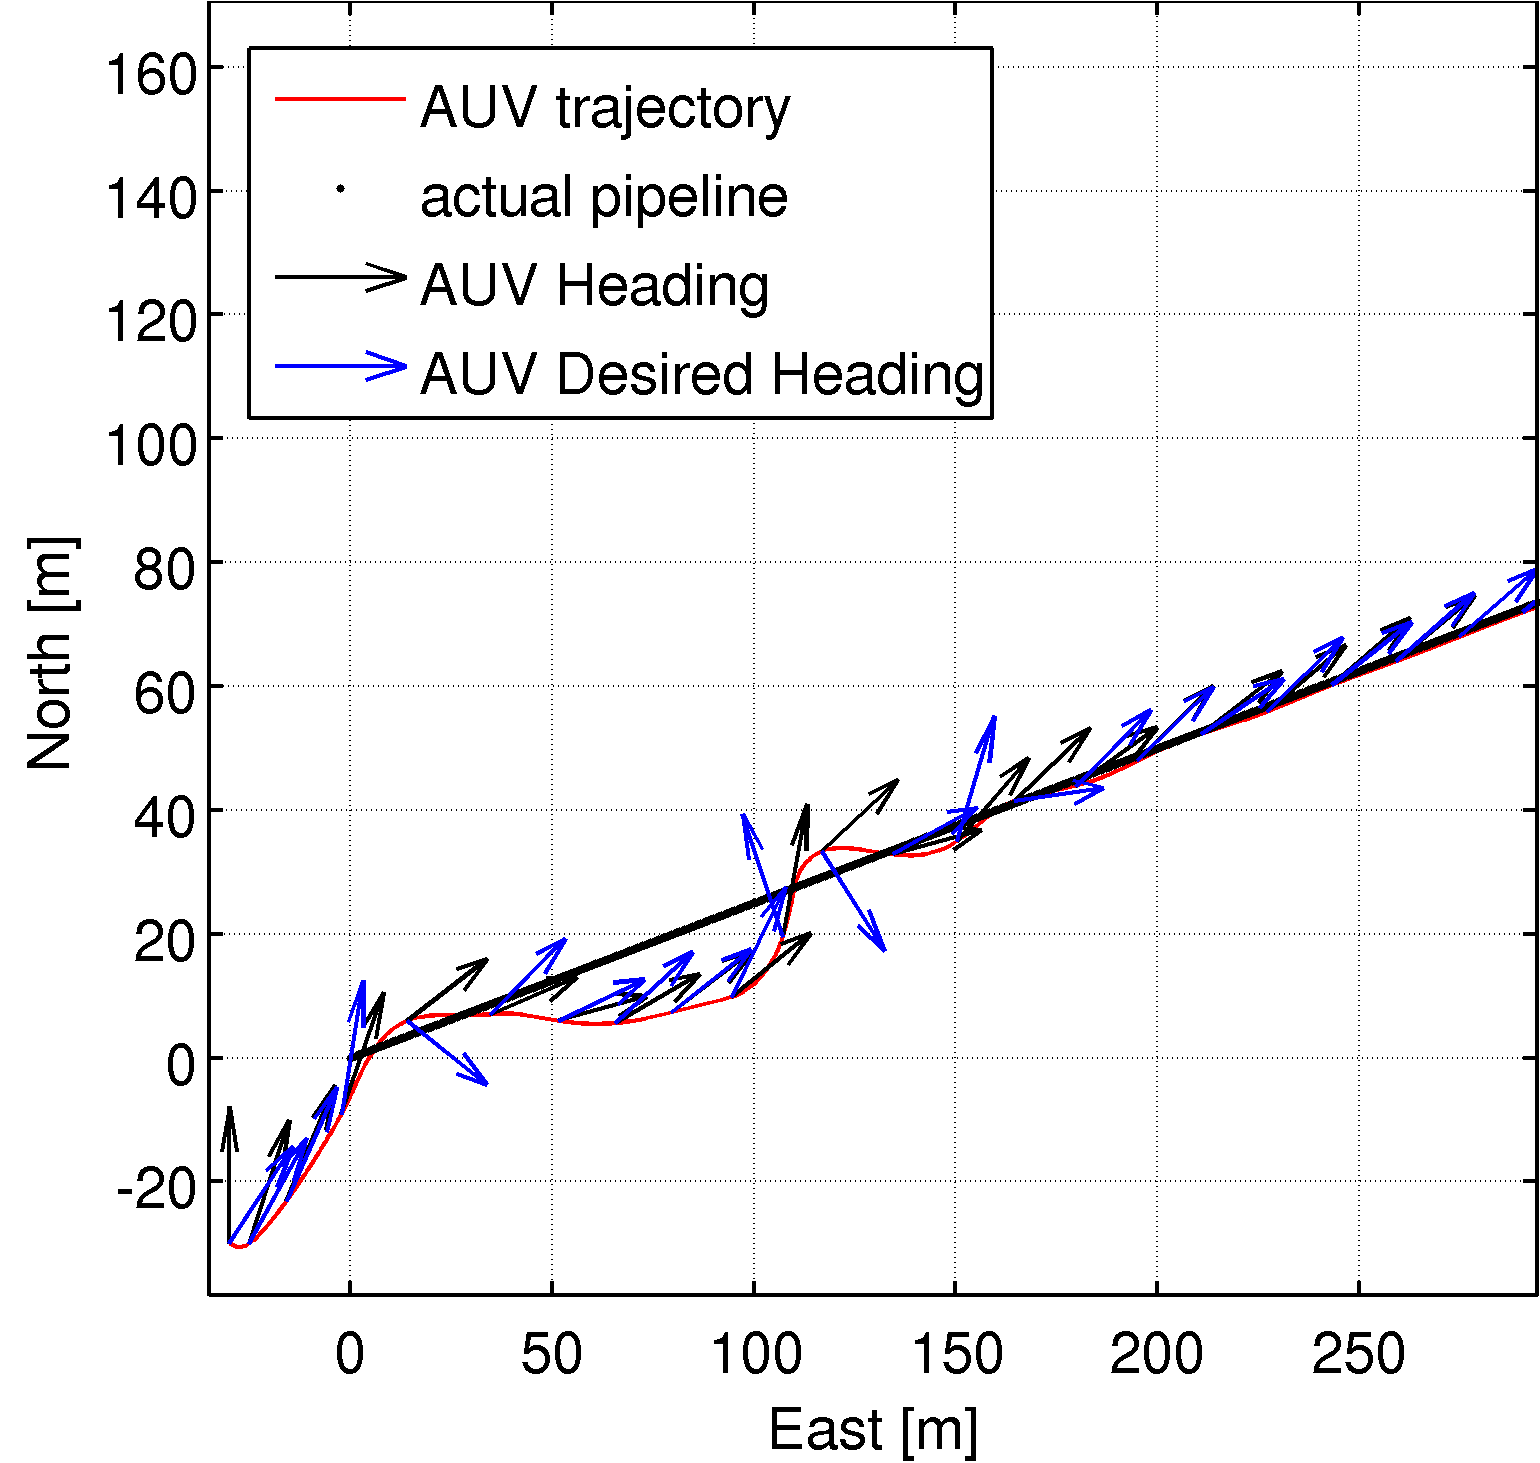
\includegraphics[width=0.5\textwidth]{pics/2nd_NE_path}} 
			\caption{Plots of the AUV Showing Trajectory, Guidance Waypoints and Heading of AUV
			second scenario}
			\label{fig:ch3_2nd_NE_plots}
		\end{figure}
		In Figure \ref{fig:ch3_2nd_NE_wpt} the search waypoints are shown. The reason for the extra
		``de-tour'' away from the pipeline are because of the short time delay befor considering the
		pipeline lost. As seen in the first Scenario there are oscilations in the heading reference.
		This cuases the AUV to drift off the pipeline trajectory and therefor lose visual contact
		with it. The system considers the pipeline as lost and generates a search pattern, the
		``divergent zig-zag'' spoken of in Chapter \ref{subsec:ch2_searchpattern}. The time before
		going into search mode are set to 25 seconds.

		\begin{figure}[htbp]
			\centering
			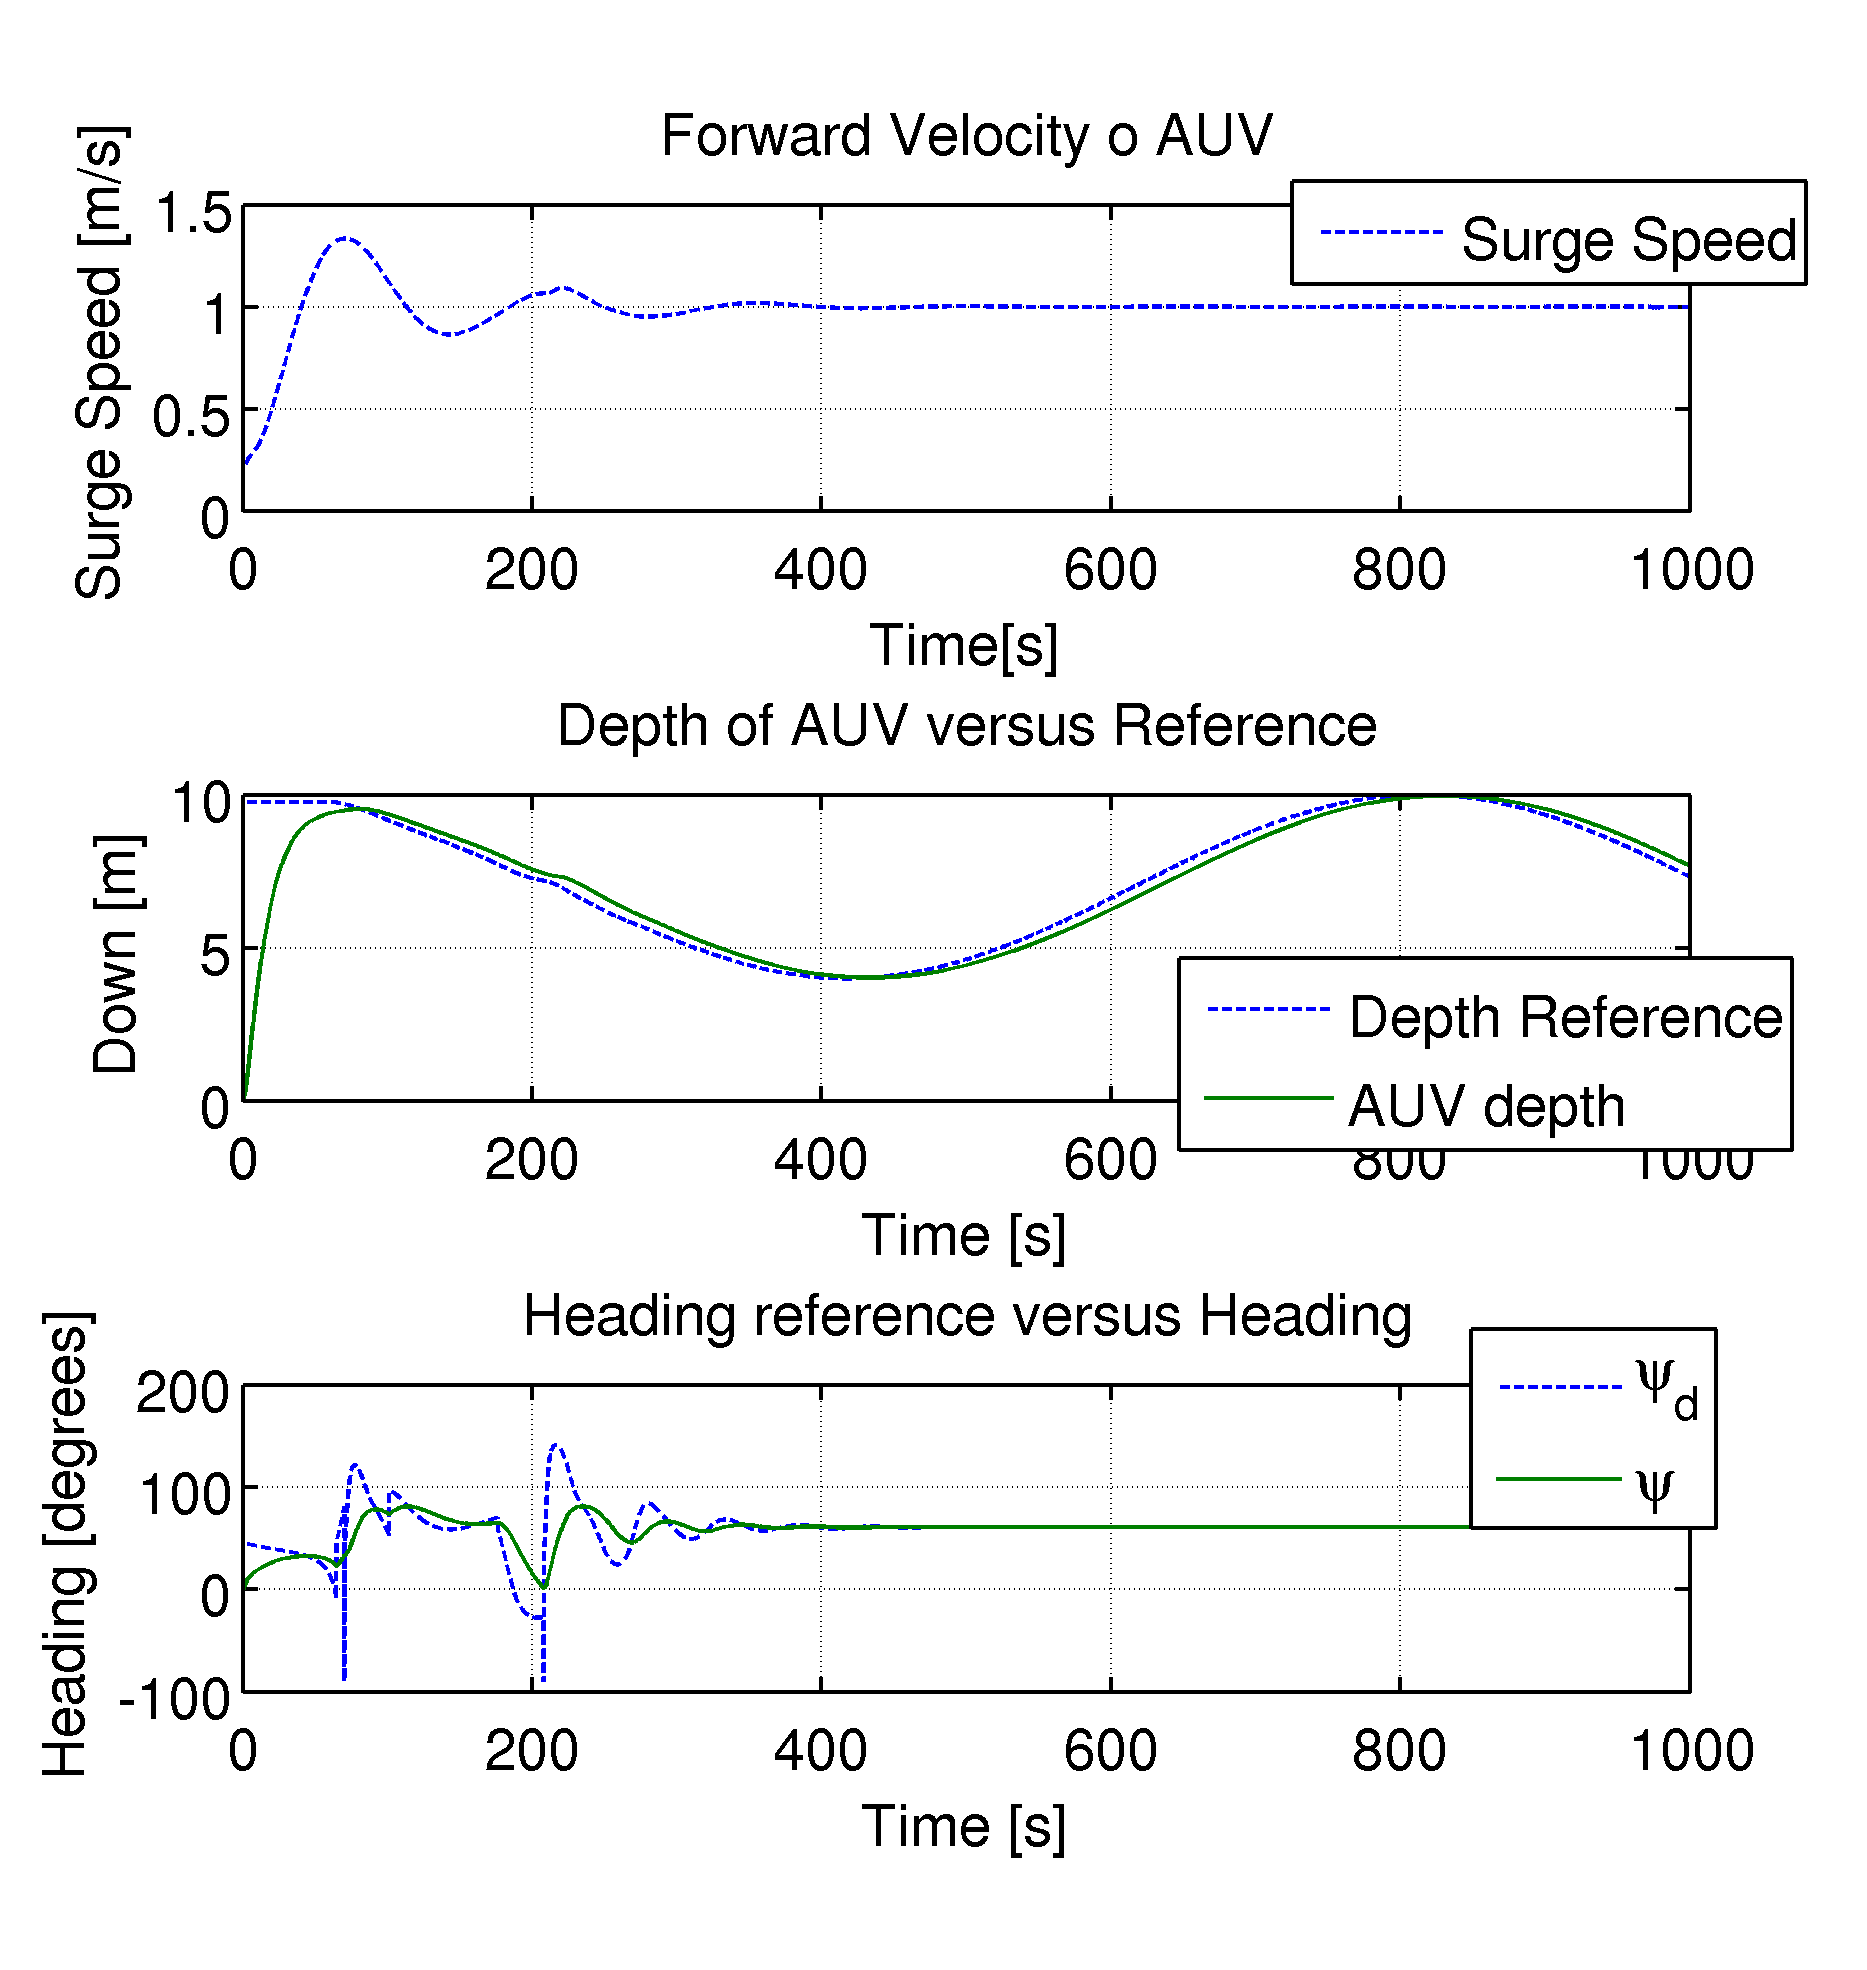
\includegraphics[width=0.70\textwidth]{pics/2nd_uDpsi}
			\caption{Surge-, Depth- and Heading- Reference with Current influence second scenario}
			\label{fig:ch3_2nd_uDpsi}
		\end{figure}
		When current are introduced the AUV heading are ``leaned'' toward the current. In Figure
		\ref{fig:ch3_2nd_NE_path} the current are coming from north-west, corresponding to
		the upper right corner in the figure. This current will try to push the
		AUV off the pipeline. The guidance system answers this disturbance by adjusting the heading
		reference towards the current. This is one of the reasons why the lookahead distance are
		chosen small, because of this the AUV will no drift far away from the pipeline. Since the
		current is constant, a equilibrium is achieved between the desired heading and the
		current. The heading converges towards around $60^{\circ}$ instead of the pipeline direction
		of $75^{\circ}$.

		The AUV are not directly on top of the pipeline anymore, but it is not desirable to be exactly
		over the pipeline all the time. To strictly control the AUV to lay exactly over the pipeline
		would use up much of the limited power supply. The objective of the AUV are not to stay
		exactly over the pipeline but to provide good pictures and sensor data for later inspections 
		by humans, because it might be easier to analyse a stable picture than a tightly regulated
		motion which might cause a noisy picture. 

		%\begin{figure}[htbp]
		%	\centering
		%	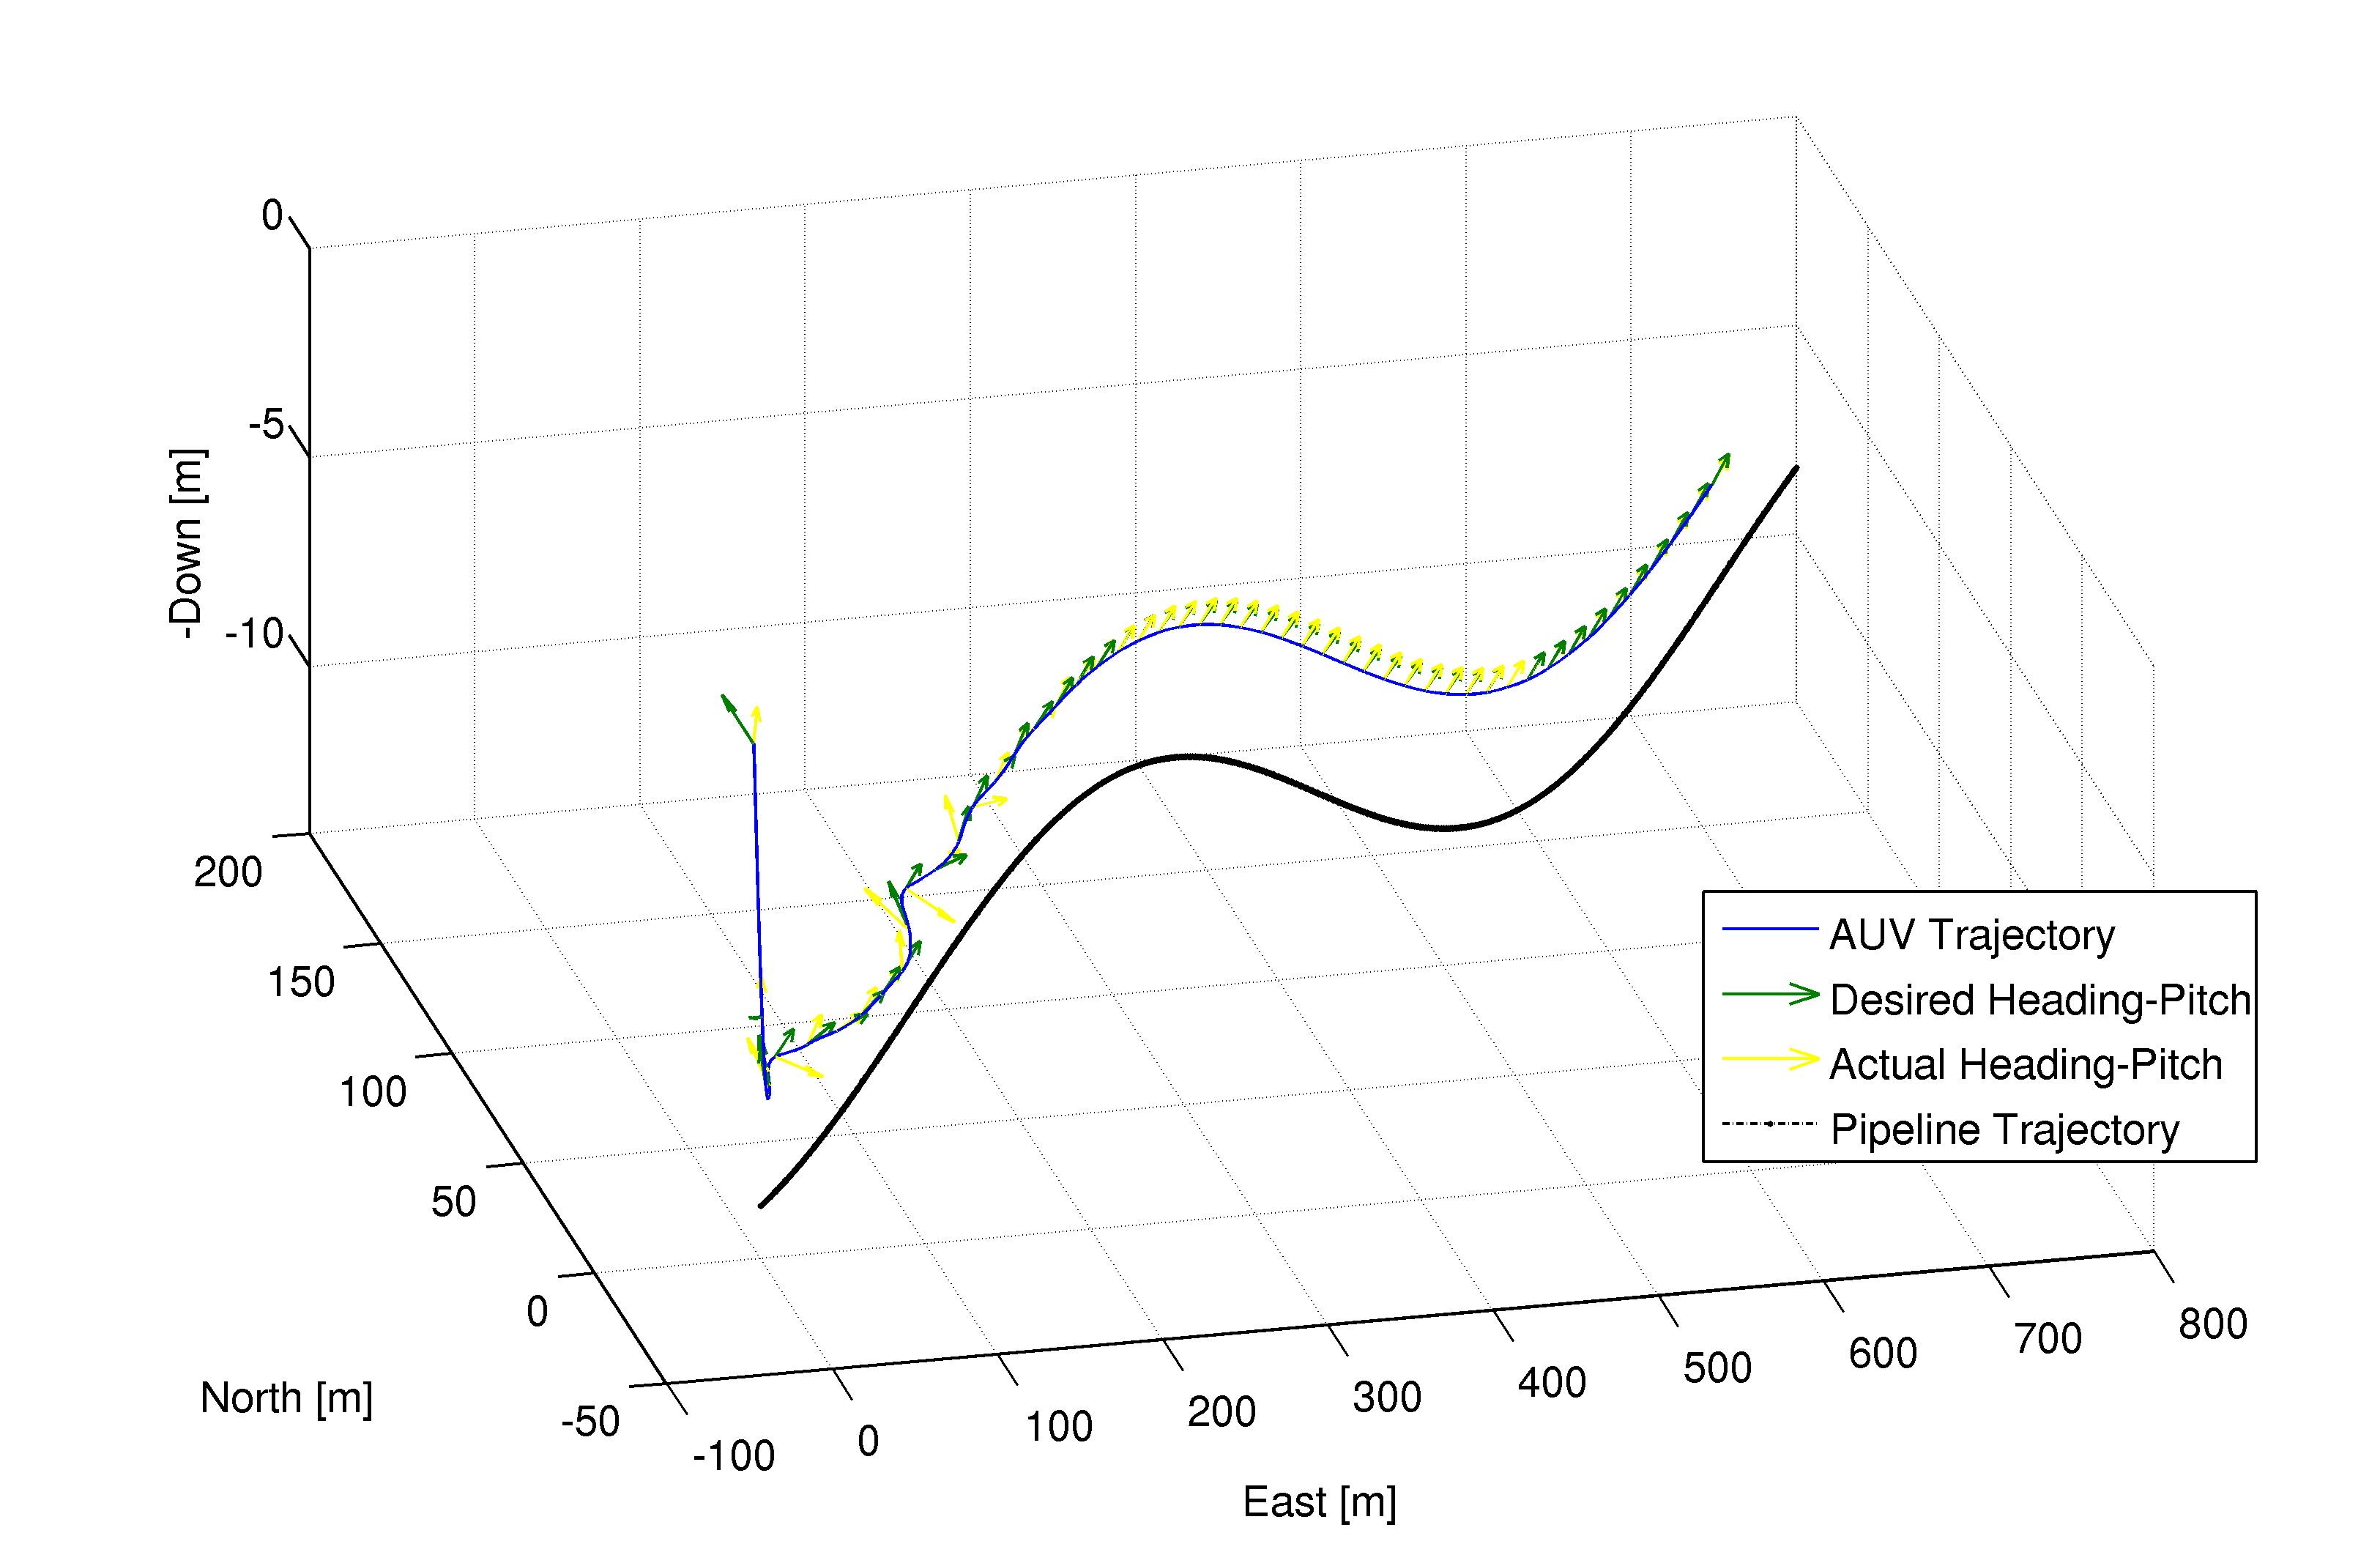
\includegraphics[width=0.95\textwidth]{pics/2nd_3d_plot}
		%	\caption{3D plot of the AUV Movement}
		%	\label{fig:ch3_2nd_3d_plot}
		%\end{figure}
		%In Figure \ref{fig:ch3_2nd_3d_plot} the 3D trajectory of the AUV are shown, togheter with the
		%actual pipeline trajectory. 
	

	\subsection{3$^{\mathrm{rd}}$ Scenario}
		The setup for this scenario, is a simulated burrial of the pipeline at apporximtley $50$
		meters North and $200$ meters East. At this point the camera looses track of the pipeline. The
		guidance system will command the AUV to continue following the predicted pipeline until some
		time limit are reached. This time limit are set to $60$ seconds. From Figure
		\ref{fig:ch3_3rd_NE_plots} it can be seen that the AUV follows the predicted pipeline for
		about $50$ meters and then engages in the predetermined search pattern.
		\begin{figure}[htbp]
			\centering
			\subfigure[NE Path with	Waypoints]{\label{fig:ch3_3rd_NE_wpt}
				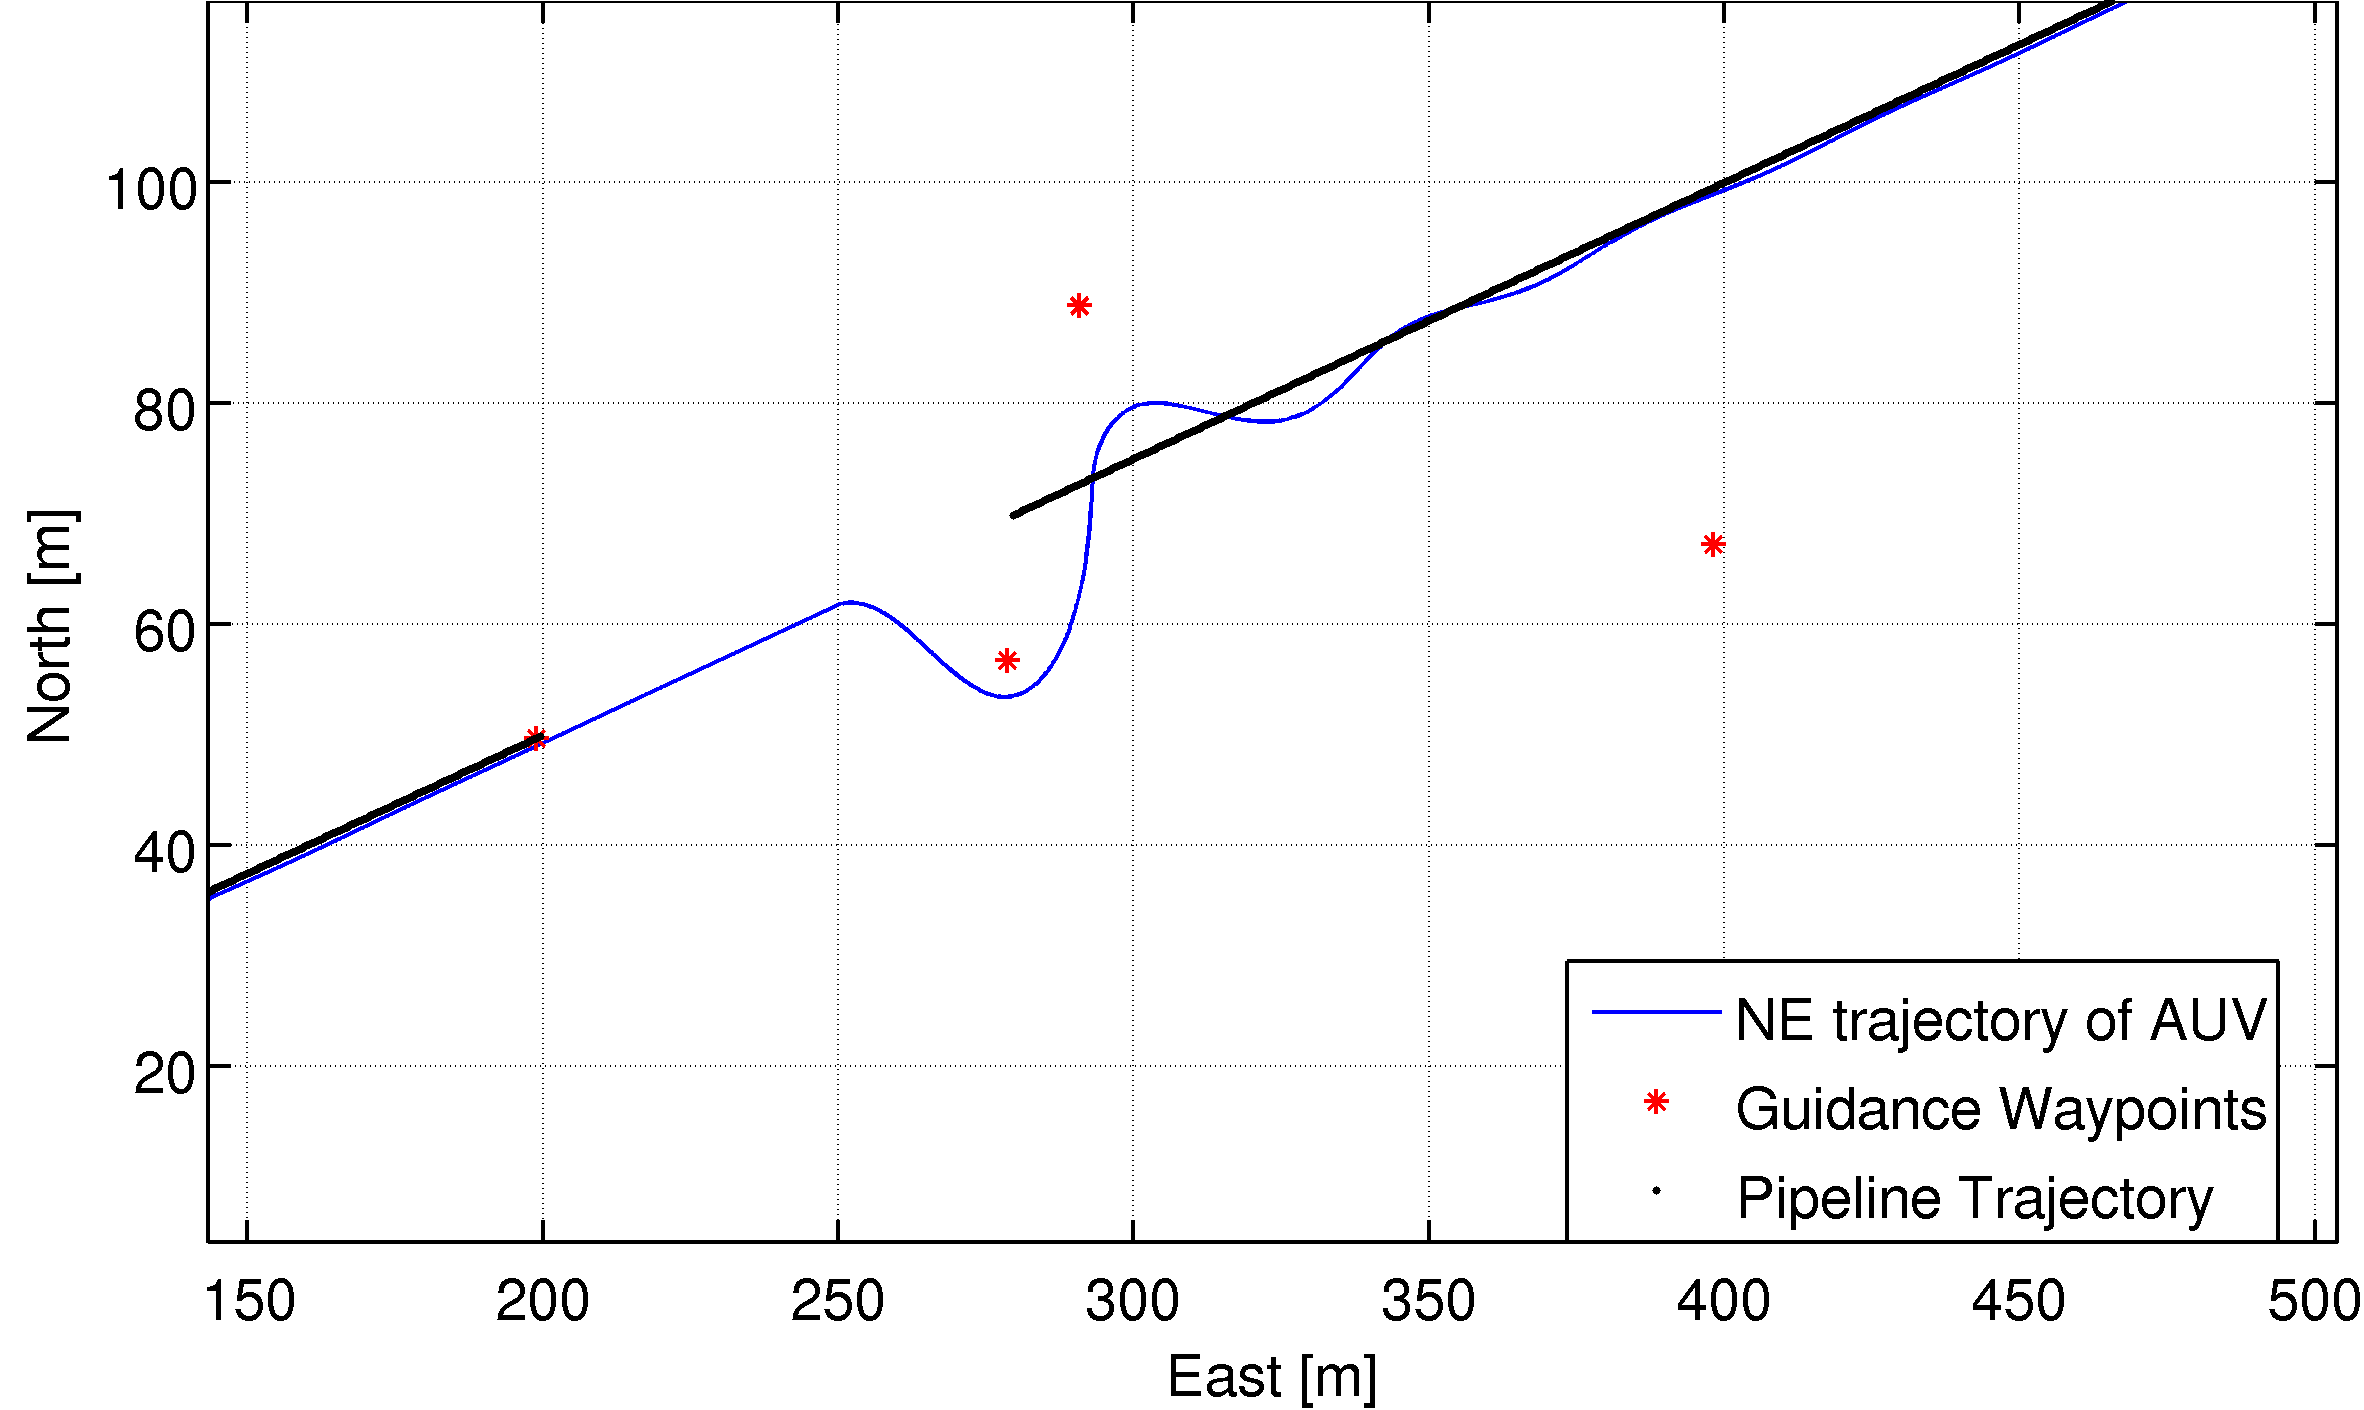
\includegraphics[width=0.7\textwidth]{pics/3rd_NE_wpt}}
			\subfigure[NE path with	Heading]{\label{fig:ch3_3rd_NE_path}
				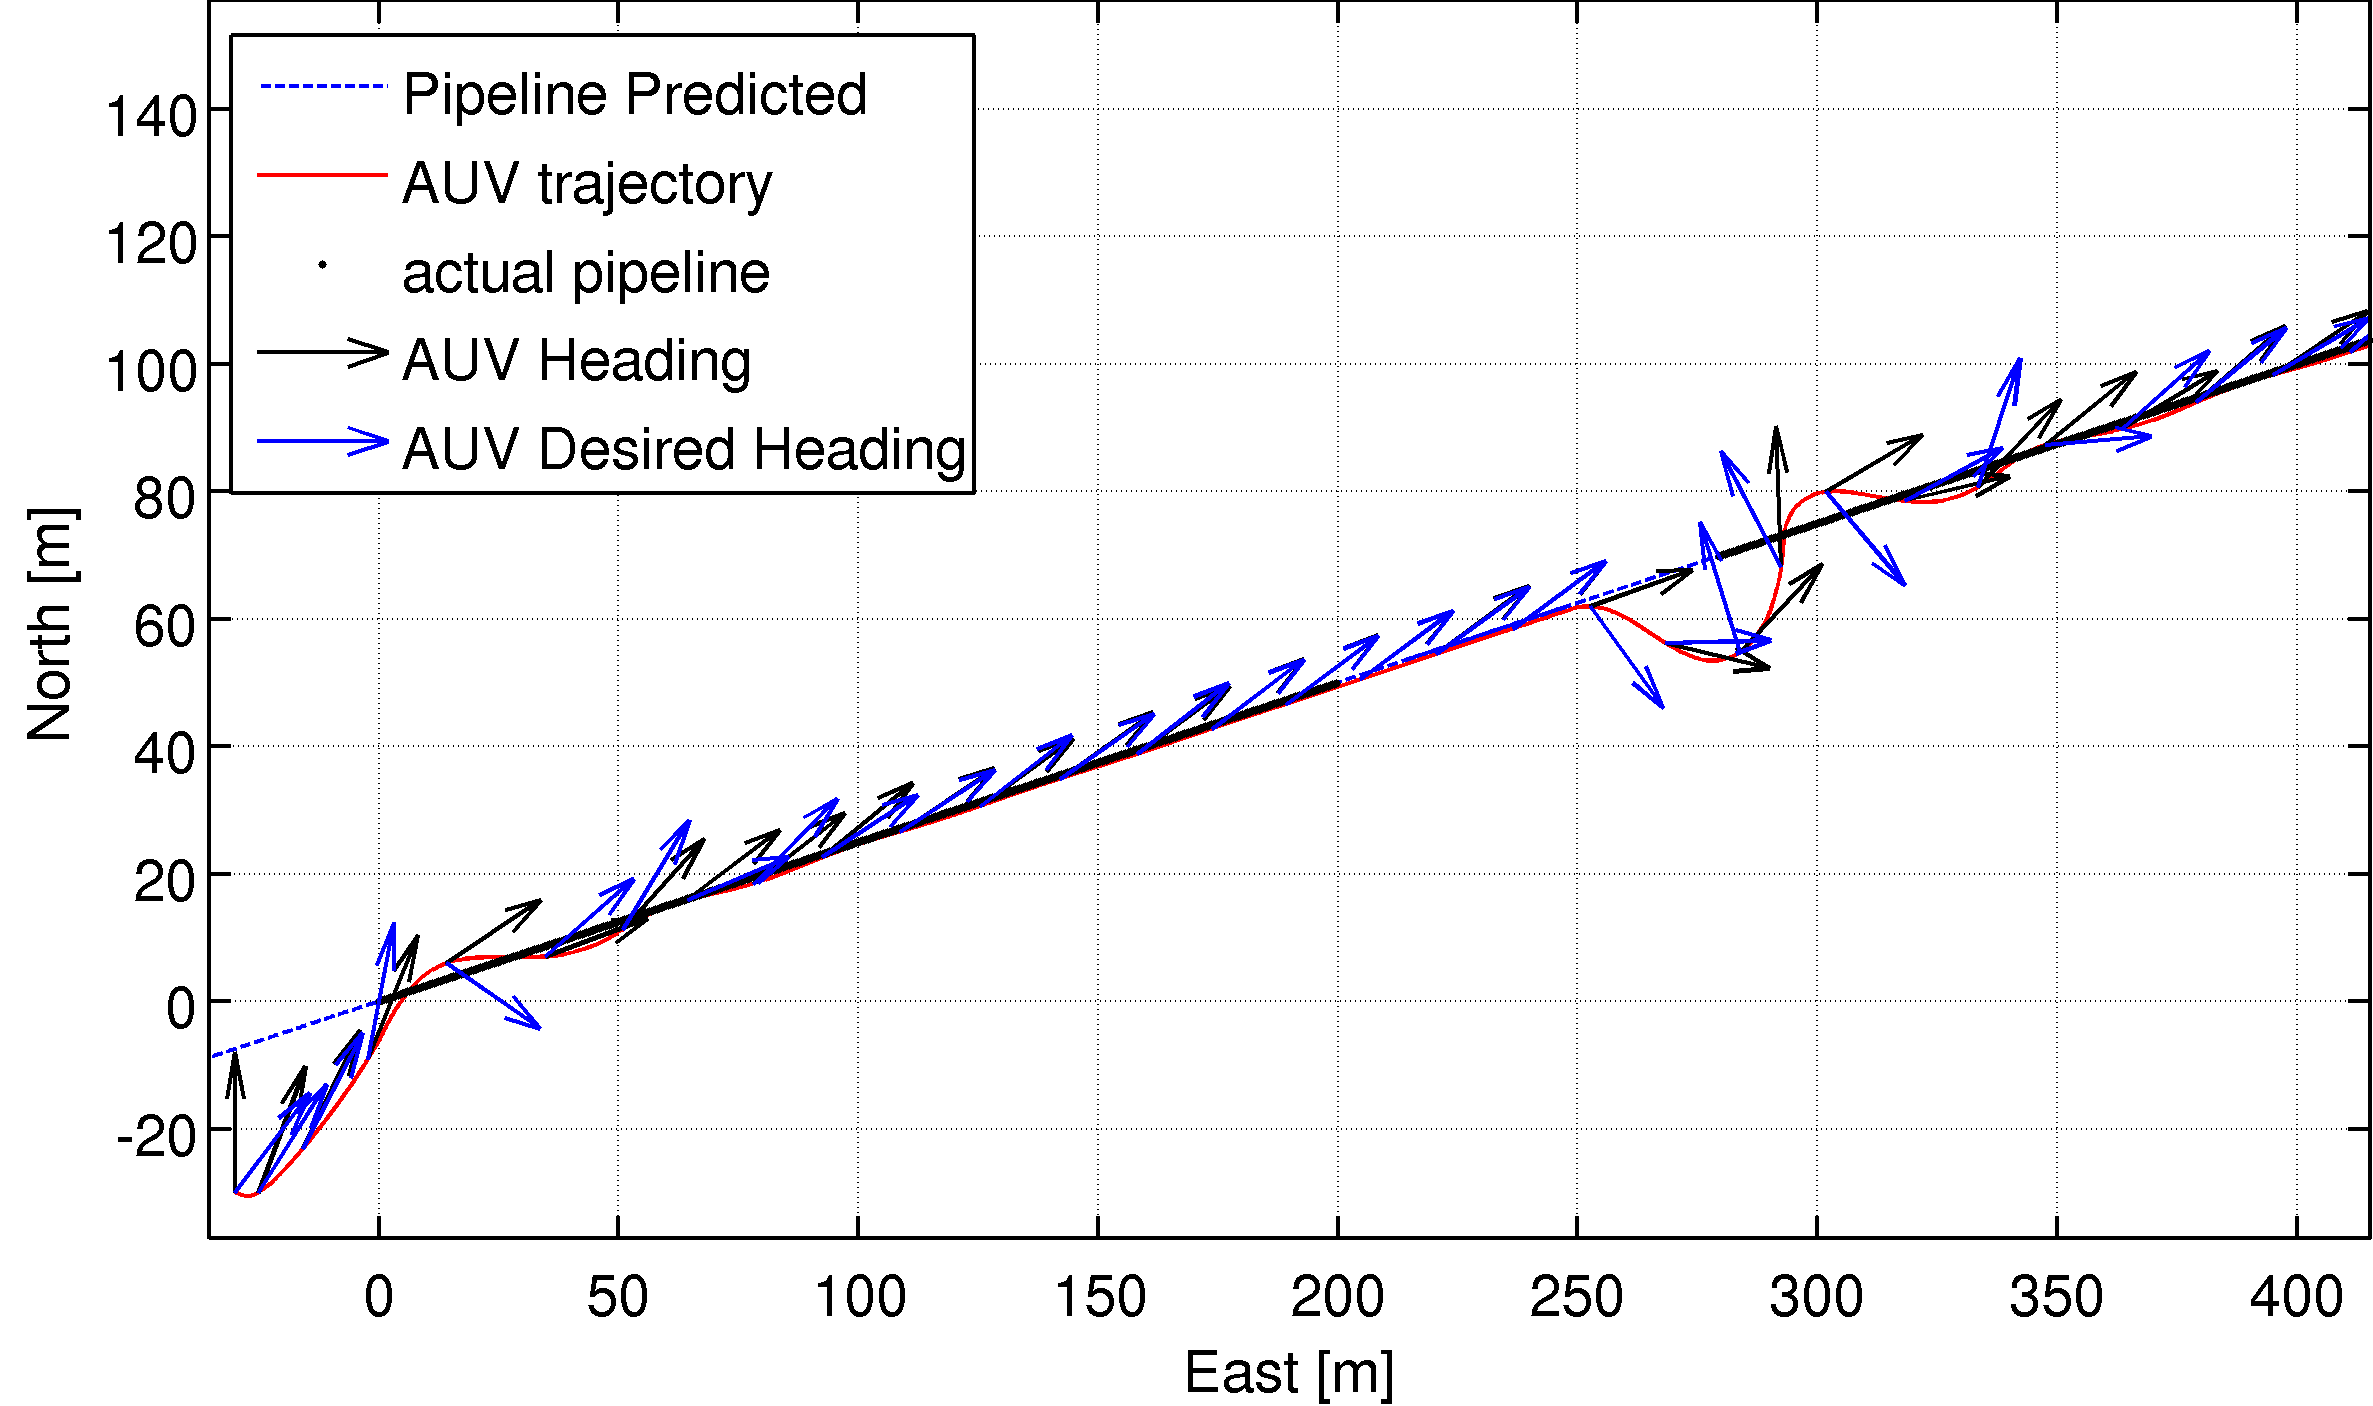
\includegraphics[width=0.7\textwidth]{pics/3rd_NE_path}} 
			\caption{Plots of the AUV Showing Trajectory, Guidance Waypoints and Heading of AUV
			for the 3$^{\mathrm{rd}}$ Scenario}
			\label{fig:ch3_3rd_NE_plots}
		\end{figure}
		
		The objective to follow the predicted pipeline is ofcourse to get back on track at the end of
		the burried strech. Sometimes pipelines are burried on purpose to seal them from environmental
		erotion, that shorten the lifetime of the pipeline. Sometimes this happens unintended. In
		either case the need for more sensors which can penetrate the sea bottom and locate the
		pipeline are needed. 

		There are no turning trajectory generator implemented at this point, and will not be used in
		the next scenarios either.
		
	
	
	\subsection{4$^{\mathrm{th}}$ Scenario}
		The fourth Scenario is to demonstrate the capabilities for the AUV to aquiere the pipeline
		when it is offset from where it was thought to be. 
		
		\begin{figure}[htbp]
			\centering
			\subfigure[NE Path with	Waypoints]{\label{fig:ch3_4th_NE_wpt}
				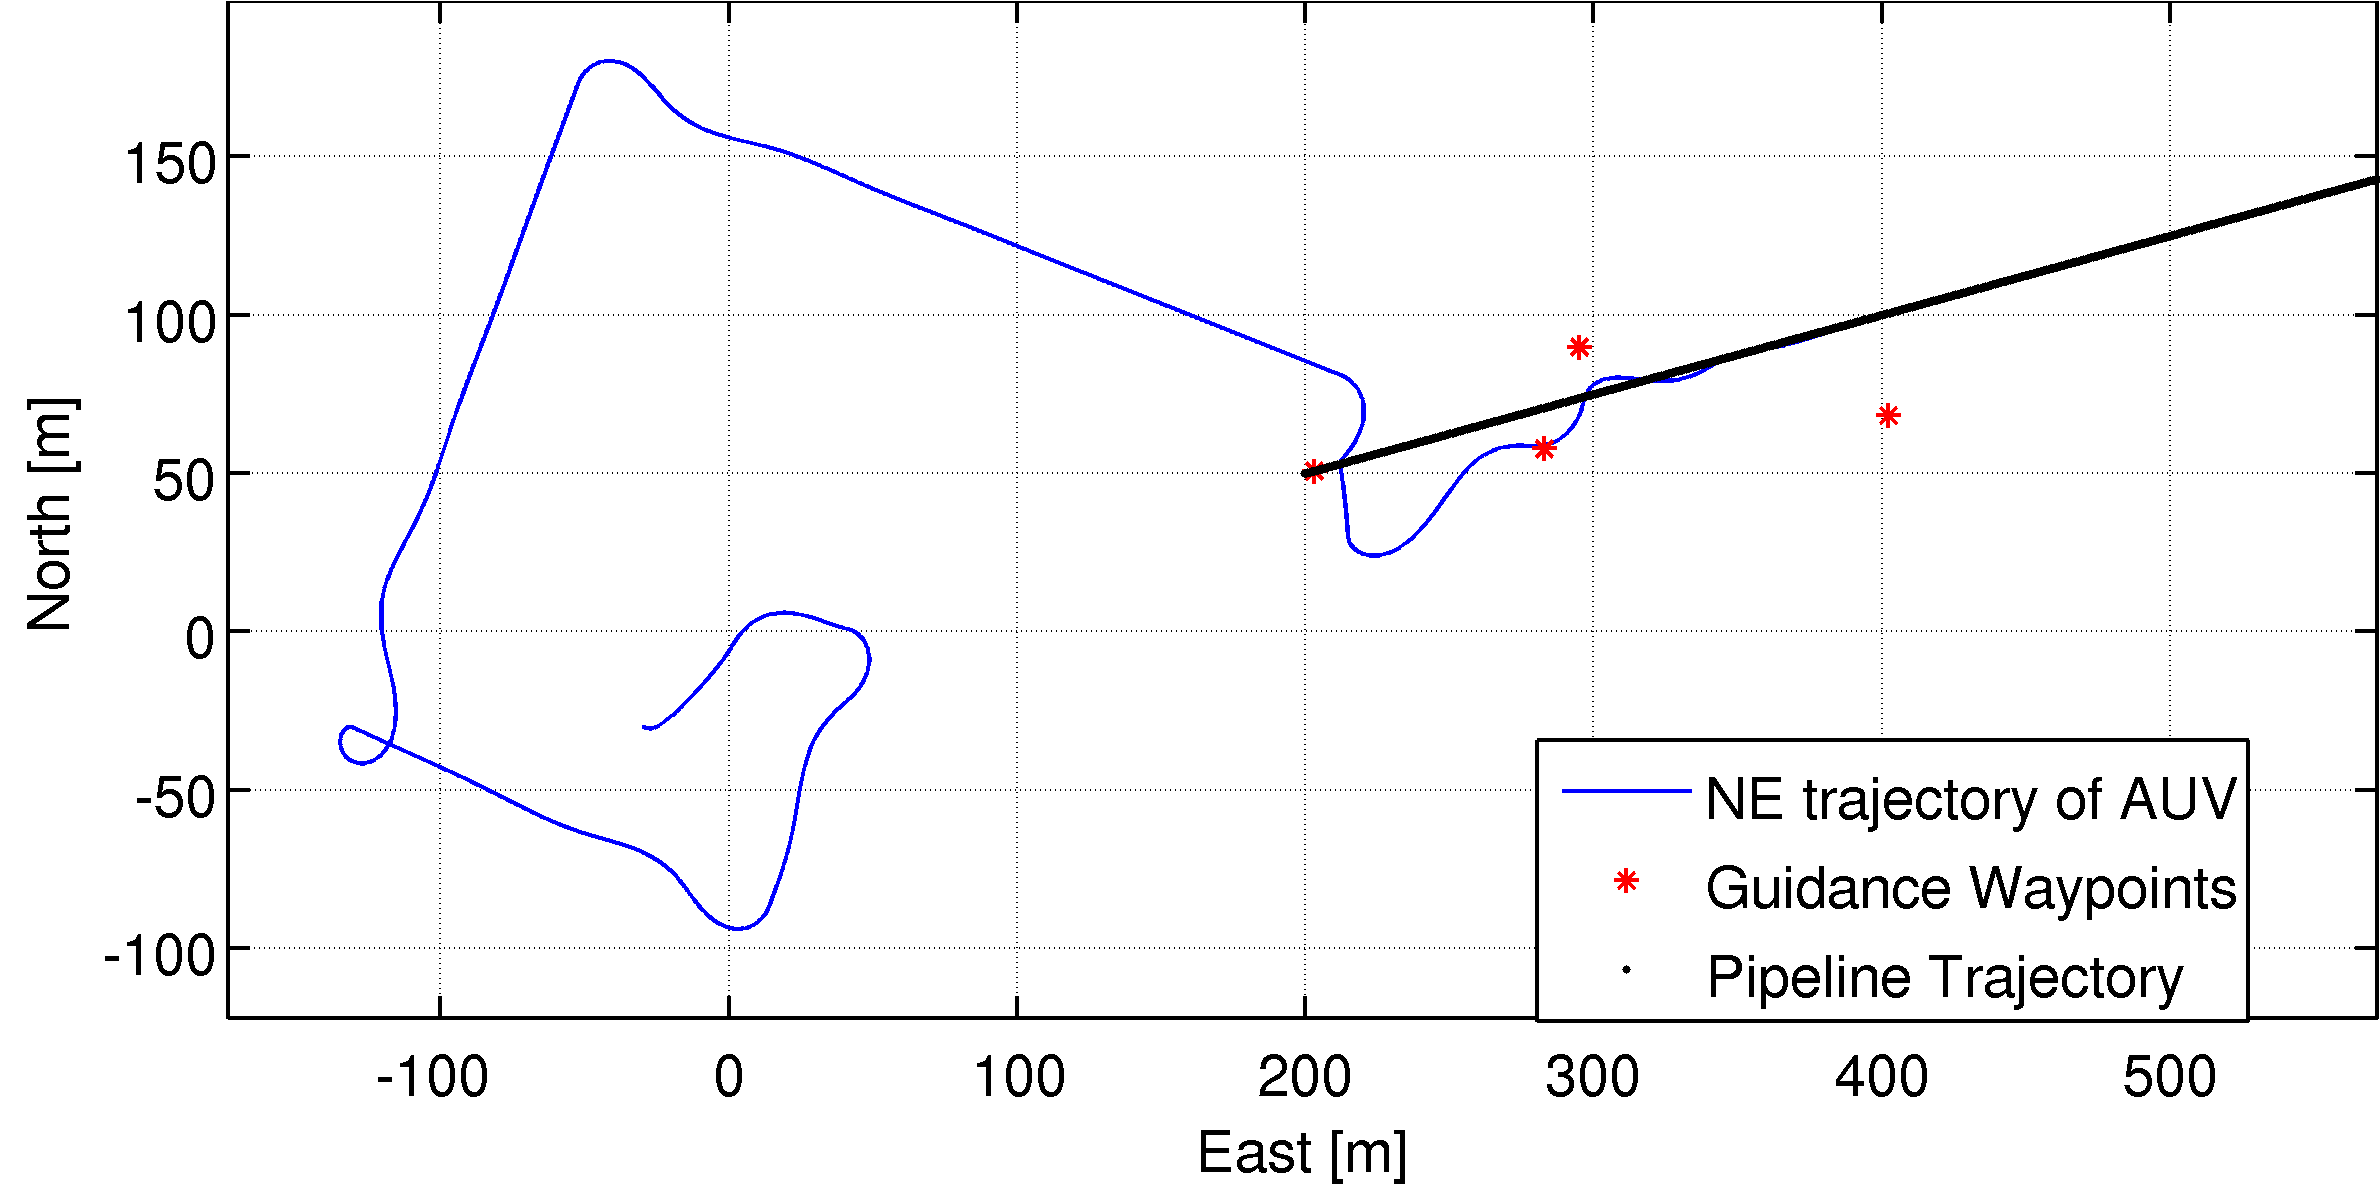
\includegraphics[width=0.8\textwidth]{pics/4th_NE_wpt}}
			\subfigure[NE path with	Heading]{\label{fig:ch3_4th_NE_path}
				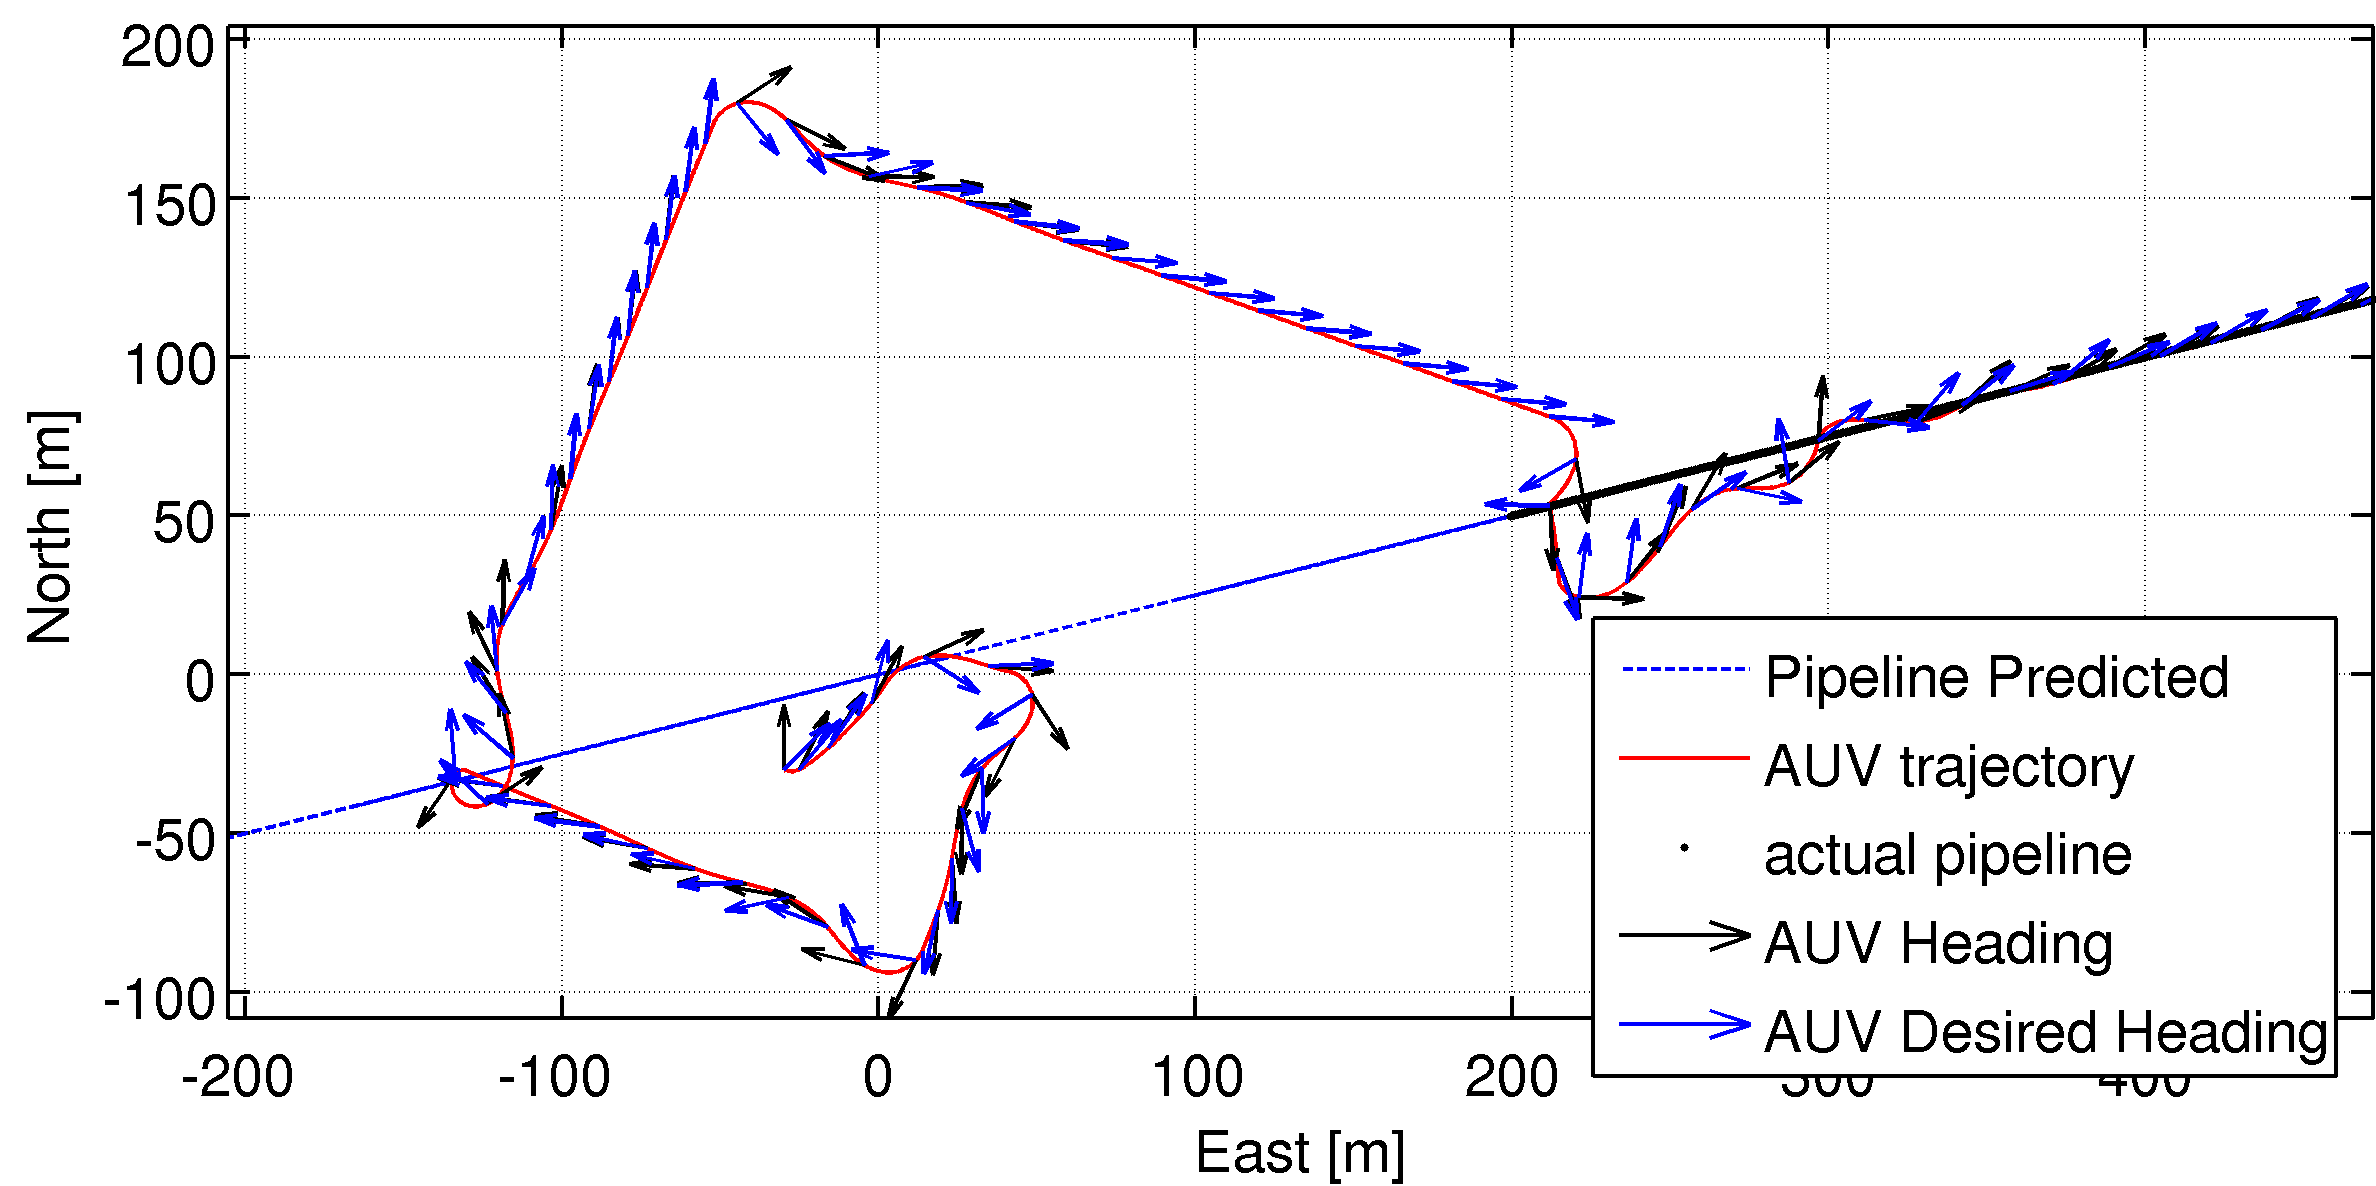
\includegraphics[width=0.8\textwidth]{pics/4th_NE_path}} 
			\caption{Plots of the AUV Showing Trajectory, Guidance Waypoints and Heading of AUV
			for the 4$^{\mathrm{th}}$ Scenario}
			\label{fig:ch3_4th_NE_plots}
		\end{figure}
		When the AUV reaches the initial position where the pipeline were ment to be. It does not make
		contact with it there, then engages in a spiral search pattern. This search pattern are
		administered by waypoints and the guidance uses the straight lines between the waypoints as
		the track to follow. This causes the more polygonal look than spiral. 

		From Figure~\ref{fig:ch3_4th_NE_plots} it can be seen that the AUV sometimes takse an extra turn
		when switching between waypoint four and five. This is due to the calculation of the dersired heading
		angle. The \textit{matlab}-fucntion, \textit{atan2()} are used which outputs the angle in the
		domain $(-\pi, \pi)$. Since the output from the AUV model are defined for all values, and this
		are fed back to the controller a heading reference of 0 means that it must ``unwinde'' all
		turns it has done, because this acumulate the yaw value beyond $2\pi$. This is an
		implementation issue and is not caused by the theoretical guidance system.

		The large overshoot when the AUV have located the pipeline are due to the current. This
		pushes the AUV away from the trajectory. The current increases the velocity in a direction and
		causes the turning in that direction to be more difficult than turning the other way. This is
		a problem that is present in all applications involving measurement of heading. One cannot
		meassure more than one $360^\circ$ and care must be taken when choseing the reference. This is
		also a topic in the heading controller. The turn should be taken in the direction that is the
		shortes or free of obstacles. This is an important part of the control system, but has not
		been implemented in the current test environment. It becomes an important issue when the turn
		involves a whole revolution around the z-axis. For a human it is quite obvious which way to
		turn, but for a non-sentient machine dependent on rules, this becomes an important issue. 

		The overshoot discussed above is also a product of the relatively large course-changing
		maneuver. This can somewhat be reduces by using a turn trajectory to get the AUV on the right
		track and the same direction as the pipeline. This trajectory generation need to handle the problem
		discussed above regarding the revolution problem.
		
		\begin{figure}[htbp]
			\centering
			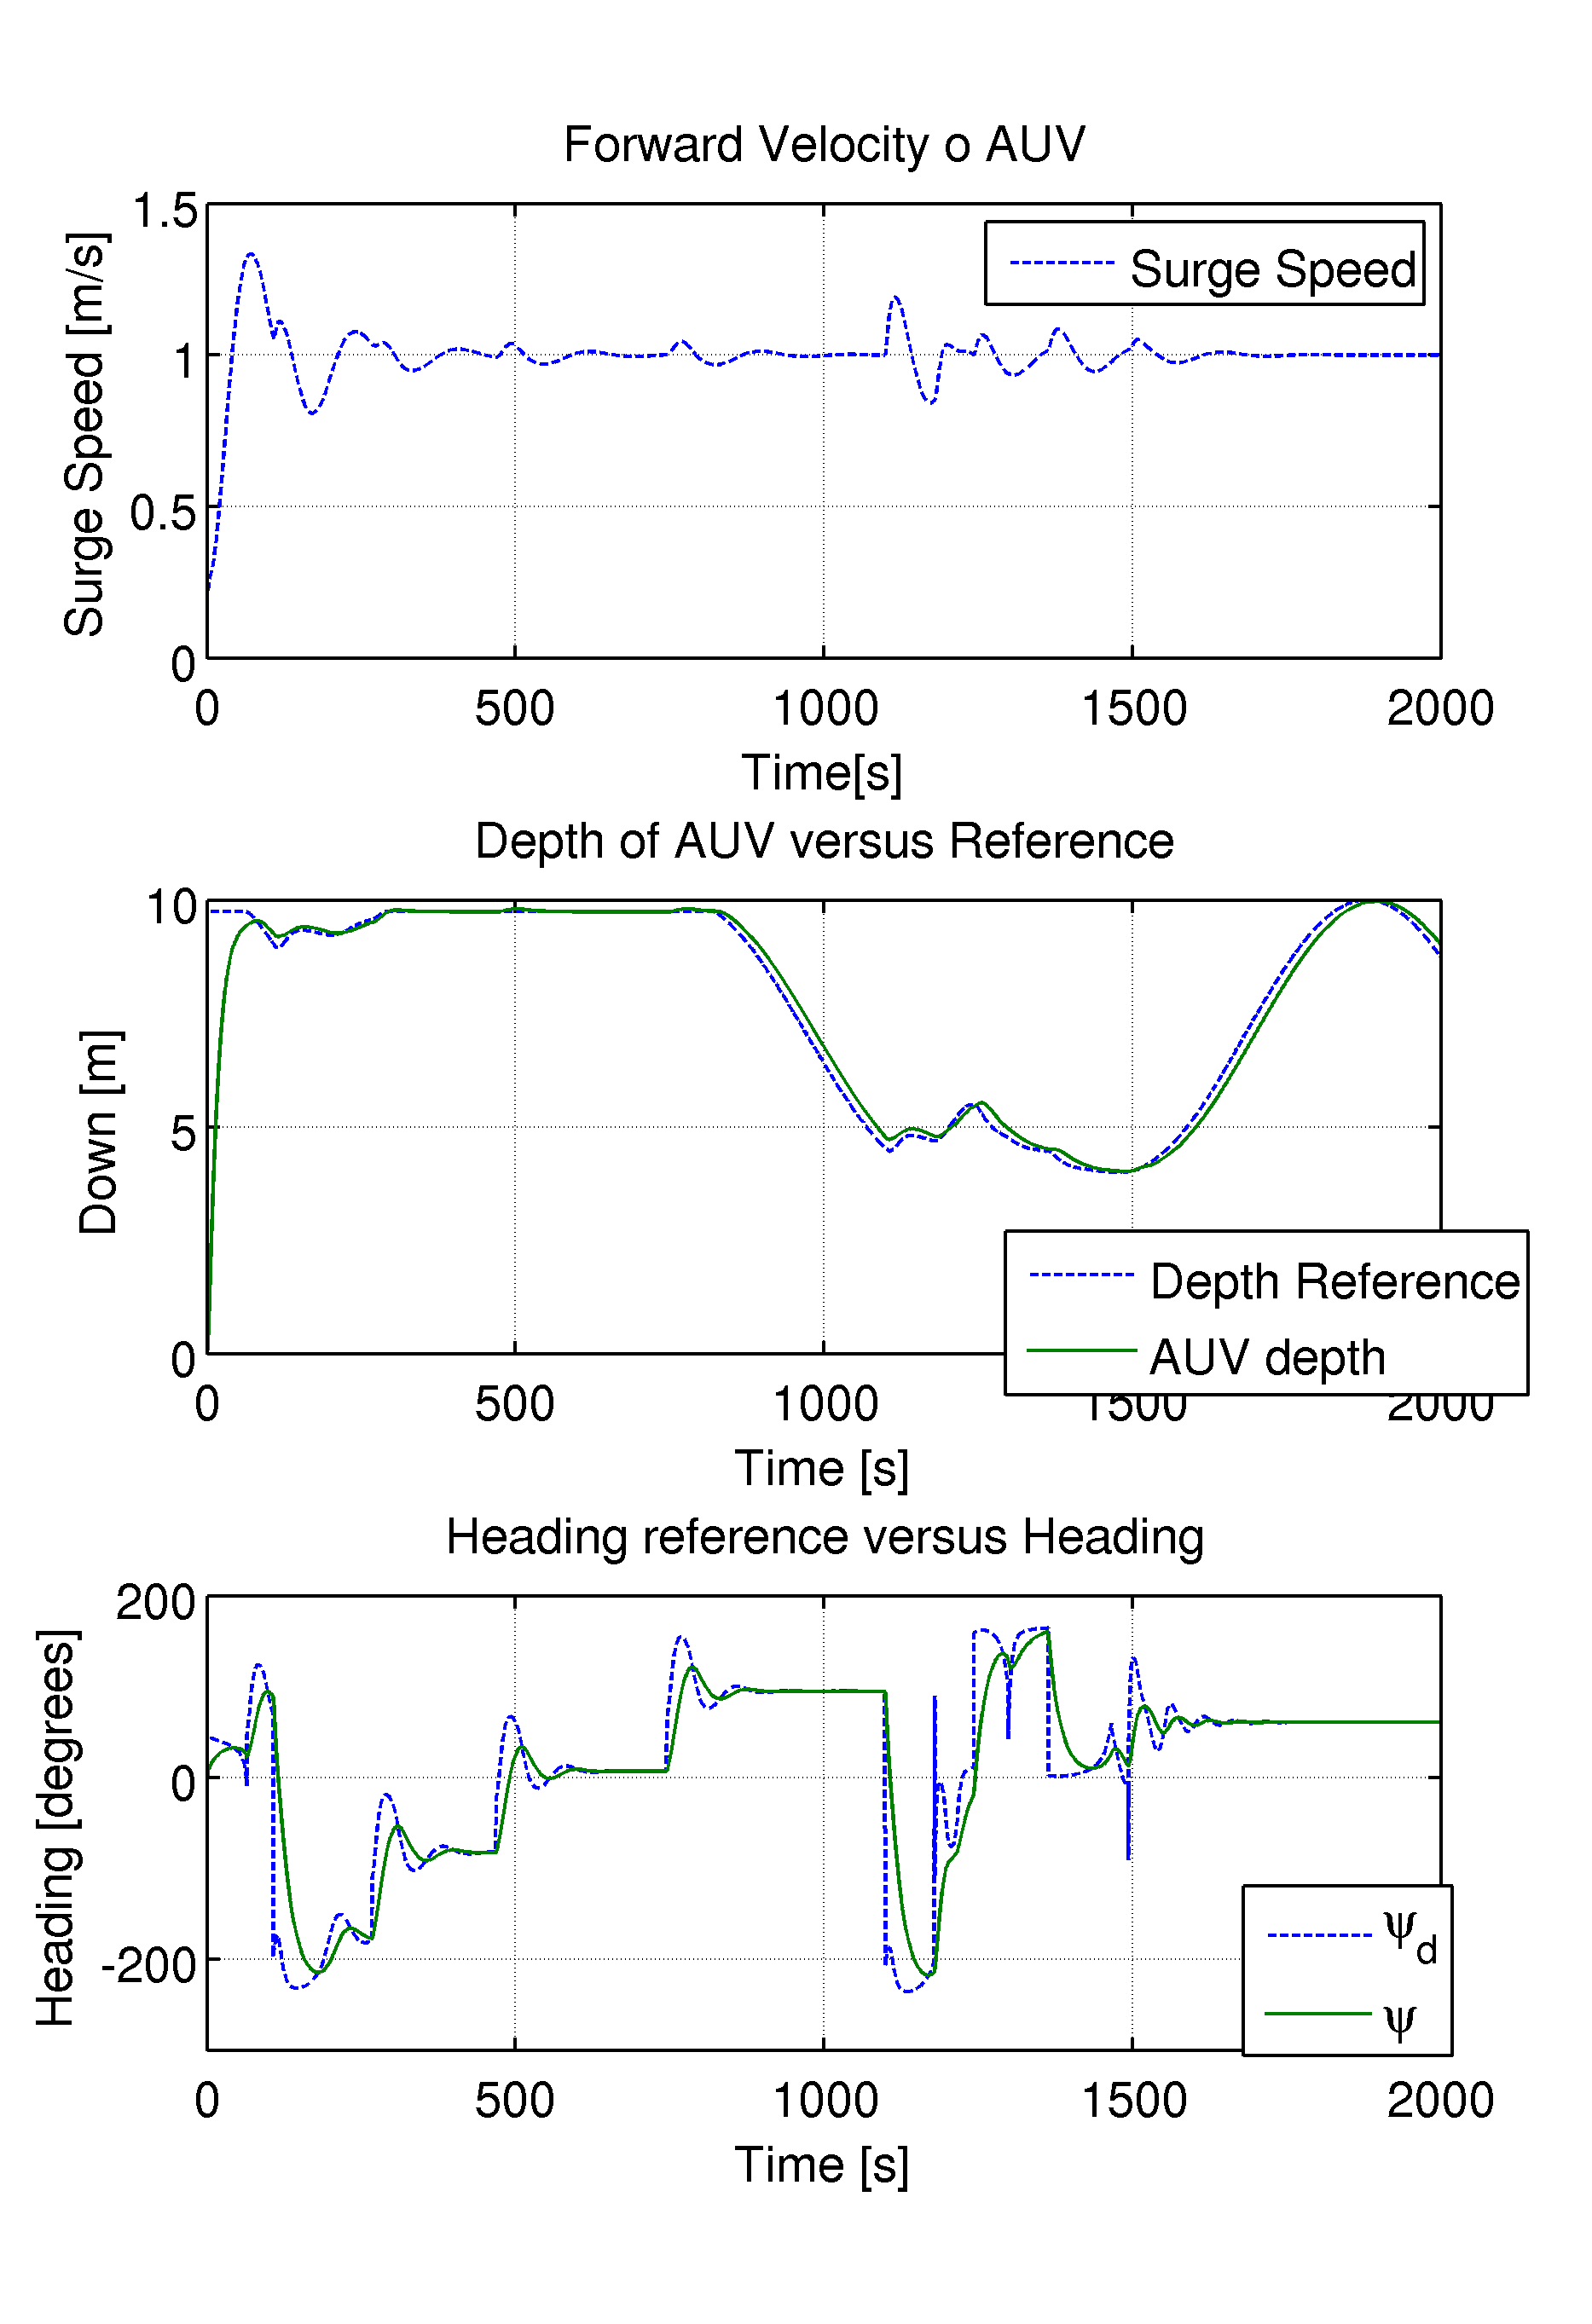
\includegraphics[width=0.70\textwidth]{pics/4th_uDpsi}
			\caption{Surge-, Depth- and Heading- Reference with Current influence for the fourth
			scenario}
			\label{fig:ch3_4th_uDpsi}
		\end{figure}
		The plots from the velocity, depth and heading references for the fourth scenario, shown in
		Figure~\ref{fig:ch3_4th_uDpsi}, are worth noting. It can be seen from the first plot in the
		figure that during large course-changing maneuvers the surge velocity first gets a overshoot
		and then decreases under the set point of 1 m/s. This is probably because of the how the
		current are included in the simulations. We see that the course changes from around $90^\circ$
		to $-200^\circ$ over short time. The surge speed changes correspondingly in the same area.
		This is becuase when the course angle are about $45^\circ$ the velocity vector are paralell to
		the current, and at $-45^\circ$ the velocity vector are still paralell but in the oposite
		direction of the current. this causes the marked changes in the surge speed seen in
		Figure~\ref{fig:ch3_4th_uDpsi}. The speed controller cannot anticipate this, and therfore does
		not ease up on the throttle.



		



\chapter{Discussion}


\section{Energy consumption}


\section{Optimal search pattern}



\section{Roll stabilization}

\chapterstyle{section}
\chapter{Conclusion}
	In this report, the topic of designing a guidance system capable of pipeline inspection 
	for the \hugin AUV have been treated. This report have looked at some basics regarding pipeline
	inspection. A literature study on how pipeline inspection can be preformed was done, and summarised in
	the report. Some basics about guidance was reviewed.

	A proposed guidance system were also designed. The system includes a flight-mode controller, a
	guidance algorithm and a Kalman filter to fuse measurements and prior knowledge about the pipeline
	together. The filter will also smooth the output from the sensors to provide a continuous reference
	for the guidance algorithm. 

	The controller designed are three independent PI-, and PID-controllers. Which were tuned according to
	stability and simulations. It is tuned with regard to velocities around $1$ m/s. Especially the heading
	controller need to be re-tuned to make it compatible with velocities higher than this.

	The behaviour of the guidance system were defined and examined. Some search patterns were discussed,
	and found that they should be customised with regard to how well the mission area are known and how
	certain the data about the pipeline are. 
	
	The system were implemented in Matlab/simulink and 4 independent simulations were run, demonstrating
	different abilities with the given guidance system. The system gave results and the given setup
	worked, also in the presence of ocean current, but are not as robust as it should be. The simulations
	were discussed with regard to energy
	efficiency and pipeline following capabilities. The most optimal path concerning energy
	optimality when the velocity are constant, is the shortest path, in most cases the linear segments
	between two points. 
	
	Whenever the AUV are tracking, the the motion above the pipeline should be constrained to be in the
	vicinity of the pipeline, but not strictly above it all the time. The primary mission of the inspection
	should be to provide good, easy-to-analyse sensor data, which in most cases include trying to maneuver 
	the AUV as smoothly as possible. 

	The camera should be aided with other sensors, such as Side Scan Sonar and Multibeam Echosounders.
	Theses sensors help with detection of the pipeline and will also provide data about the condition of
	the pipeline. 

	The strict modularity of the guidance system presented in this report allows for easy upgrades and
	improvement to the different blocks in the system. In further work with this problem the guidance
	system will be easy to upgrade, with more advanced controllers or guidance algorithms. The simulation
	environment present, gives good results.

	
\section{Further Work}
	There are much work do be done before this can be transformed into real life application.
	
	First the guidance system should handle three dimensional guidance with nonlinear paths. A possible way to 
	do this is to use unified guidance controller proposed in \cite{control-concept-AUV}. This is a 
	controller for the whole non-zero speed regime.

	The Kalman filter should be designed to include readings from other sensors like Sidescan Sonar,
	Echosounders, and other possible sensors available for the inspection mission, such as a Synthetic
	Aperture Sonar. The filter should be
	expanded to be capable of three dimensional prediction and a more sophisticated prediction might be
	used to get good results for the predictions. 
	
	It should be room for making the guidance system control the inspection velocity. If there are large 
	stretches of pipeline
	which requires little maneuvering, the speed can be increased or if there the sensors show parts of the
	pipeline which shows signs of corrosion, the inspection velocity can be slowed to give more data about
	the area.

	Develop some kind of a \textit{power} mode and \textit{economy} mode for the guidance system, where 
	the \textit{power} mode can be used when there are strong currents in the area, to help the AUV
	continue the tracking procedure, or to quickly get the AUV to the desired location. The
	\textit{economy} mode can be utilised when tracking the pipeline and environmental forces are not very
	dominating. 

	


\chapterstyle{default}

\bibliography{exbib}

%%%%%
% Many appendices
%%%%
\appendices
\appendixpage
\chapter{Moderately Important Stuff}
\section{About Appendices}
If you have many appendices, do it like this: A page signifying the start of the appendices saying ``Appendices'', then the appendices numbered A, B, C, \ldots

If you only have one appendix, do not have a page saying ``Appendices''. Have just one unnumbered chapter with title ``Appendix'', or ``Appendix: Name of Appendix''. 

\chapter{More Moderately Important Stuff}%Use for many appendices


%\backmatter
%%%%%
% Only one appendix
%%%%
\chapter{Appendix: Slightly Important Stuff}
\section{A Section}
Lorem ipsum dolor sit amet, consectetur adipisicing elit, sed do eiusmod tempor incididunt ut labore et dolore magna aliqua. Ut enim ad minim veniam, quis nostrud exercitation ullamco laboris nisi ut aliquip ex ea commodo consequat. Duis aute irure dolor in reprehenderit in voluptate velit esse cillum dolore eu fugiat nulla pariatur. Excepteur sint occaecat cupidatat non proident, sunt in culpa qui officia deserunt mollit anim id est laborum.%Use if you only have on appendix

\end{document}
